\documentclass{book}


% Page size
\usepackage[a5paper]{geometry}


% Font
\usepackage{fontspec}
\setmainfont{Clara}


% Typesetting
\usepackage{microtype}


% Colors
\usepackage[dvipsnames]{xcolor}
\definecolor{darkgray}{gray}{0.35}


% Languages
\usepackage[english, latin]{babel}


% Figures
\usepackage{graphicx}


% Initials
\usepackage{lettrine}


% Columns
\usepackage{paracol}


% Line spacing
\usepackage{setspace}


% Paragraph spacing and indents
\setlength{\parskip}{0.75\baselineskip}
\setlength{\parindent}{0pt}


% Decorative borders
%\usepackage[object=vectorian]{pgfornament}
%\usepackage{tikz}


% Remove page numbers when using cleardoublepage
\usepackage{emptypage}


% Margin notes inside text columns
\usepackage{wrapfig}


% Math
\usepackage{amsmath}


% Put page number at bottom
\pagestyle{plain}



\begin{document}

\pagenumbering{roman} 

{\fontsize{11}{11} \selectfont

\begin{titlepage}
\begin{center}
{\bfseries \lsstyle
{\Large CRONICA}

\vspace{0cm}

{\color{BrickRed} \Huge JOCELINI \\ \vspace*{0.5cm} DE BRAKELONDA,}

\vspace{0.4cm}

{\Large DE REBUS GESTIS SAMSONIS}

\vspace{0.2cm}

{\Large ABBATIS MONASTERII}

\vspace{0.4cm}

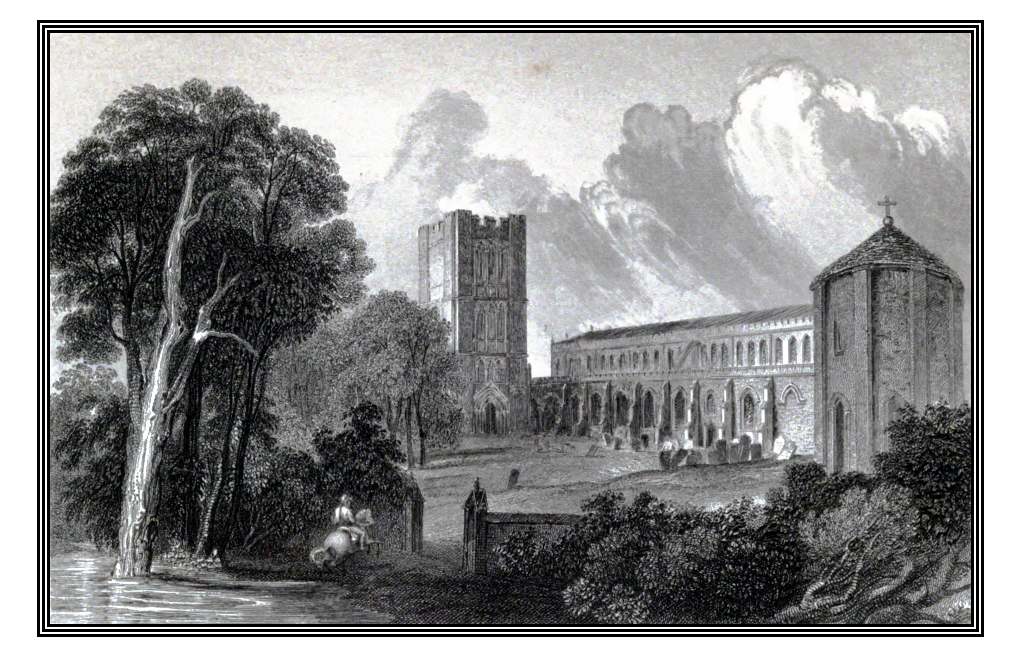
\includegraphics[scale=0.37]{fig/abbey.png}

\vspace{0.4cm}

{\color{BrickRed} \Huge SANCTI \AE{}DMUNDI.}

\vspace{0.2cm}

}
\end{center}
\end{titlepage}


\thispagestyle{empty}
\begin{center}

{\setlength{\parskip}{3mm}

Cronica de rebus gestis Samsonis abbatis
 
(Harl.\ MS.\ 1005 ff.\ 127r--170v)

Jocelin of Brakelond

\vspace*{5mm}

{\small \emph{Compiled, reset and reprinted \&c.}}

R.\ Creswell

Oxford

MMXXI

}

\end{center}

\vfill

{\setlength{\parskip}{1mm} \small

\emph{Frontispiece---}

G.\ F.\ Sargent and J.\ C.\ Varrall in \emph{The Book of Shakespeare Gems: In a Series of Landscape Illustrations of the Most Interesting Localities of Shakespeare's Dramas}, Bohn, London, \oldstylenums{1846}.

\vspace{0.4cm}

\emph{Latin text---}

Ed.\ T.\ Arnold: \emph{Memorials of St.\ Edmund's Abbey}, Vol.\ \oldstylenums{1}, Rerum Britannicarum Medii \AE{}vi Scriptores, The Lords Commissioners of Her Majesty's Treasury, Under the Direction of the Master of the Rolls, London, \oldstylenums{1890}.


\vspace{0.4cm}

\emph{English translation, introduction and footnotes---}

Trans.\ ed.\ L.\ C.\ Jane, intr.\ Abbot Gasquet: \emph{The Chronicle of Jocelin of Brakelond, Monk of St.\ Edmundsbury: A Picture of Monastic and Social Life in the XII{\tiny TH} Century}, Chatto \& Windus, London, \oldstylenums{1907}.

}


\newpage

\thispagestyle{empty}
\begin{center}

\hspace{0pt}
\vfill

{\setstretch{1.1}

\parbox{5.5cm}{
\makebox[0pt][r]{\emph{``}}{\emph{Fly, noble English, you are bought and sold;\\
Unthread the rude eye of rebellion\\
And welcome home again discarded faith.\\
Seek out King John and fall before his feet;\\
For if the French be lords of this loud day,\\
He means to recompense the pains you take\\
By cutting off your heads: thus hath he sworn\\
And I with him, and many moe with me,\\
Upon the altar at Saint Edmundsbury;\\
Even on that altar, where we swore to you\\
Dear amity and everlasting love.''}
}
}
}

\vfill
\hspace{0pt}

\end{center}

\cleardoublepage

\begin{center}


\hspace{0cm}\vspace{1.4cm}

\parbox{8cm}{
{\scshape
A veritable monk of Bury St.\ Edmunds is worth attending to, if by chance made visible and audible. Here he is; and in his hand a magical speculum, much gone to rust, indeed, yet in fragments still clear; wherein the marvellous image of his existence does still shadow itself, though f\vphantom iitfully, and as with an intermittent light.\\
}

\hspace{0pt}\hfill Carlyle --- \emph{Past and Present}.
}

\end{center}

\vspace{1cm}

{\setstretch{1.05}

\lettrine[lines=4]{\color{BrickRed}F}{ew} medi\ae{}val documents have exercised a greater fascination over men's minds in these latter days than ``The Chronicle of Jocelin of Brakelond.'' More than sixty years ago the publication of the Latin text of this history, by the Camden Society, attracted the attention of the great Thomas Carlyle, and furnished him with material for sketching his picture of ``The Ancient Monk,'' which occupied the entire second book of his \emph{Past and Present}. Although the modern sage in his own rugged way affected no little contempt for what he called this ``extremely foreign book,'' and for ``the monk-Latin'' in which it was written, it is evident that Jocelin's simple story of the wise, firm, yet withal gentle rule ofa medi\ae{}val abbot over a great English monastery cast a spell over him, the influence of which can be detected in every page of his delightful and almost surprisingly sympathetic account of Abbot Samson and of Edmundsbury.

In this case the \emph{Past}, as Carlyle read it in the ``Chronicle,'' was so entirely different from the \emph{Present}, as he knew it in his day, that the wonder is not that he was fascinated by it, but that he was able with its help to paint so true and living a picture and to fashion so fitting a frame in which to set it. For to him, without doubt, the story dealt with what he regarded as ``vanished existences''---``ideas, life-furniture, whole workings and ways,'' which were not only \emph{Past}, but gone beyond recall, and ``covered deeper than Pompeii with the lava-ashes and inarticulate wreck of seven hundred years!''

And indeed it cannot be denied that the ideals and aspirations, as revealed to us in the history of Abbot Samson and, so far as we know, in the life story of his biographer Jocelin, are of a higher and almost a different order to those of our modern world. To men of their calling in those far-off times, the natural and the supernatural were united and intermingled in the simplest and most ordinary way. Their very notions of the unseen world are almost sufficient to take away the breath of those whose lots have been cast in this more material and prosaic age of doubts and disbeliefs. To Samson, and Jocelin, and their fellow-monks at Edmundsbury in the twelfth century, heaven, as a great writer has said of earlier English monasticism, was hardly even ``next door.'' The future life was merely the present continued, and each man went forth to his task as it came and laboured at it day by day, not with any idea of finishing it, but only of carrying on for the span of his allotted existence. They built, and planted, and wrote till the end came, and then they went to heaven and others stepped into their places and took up the common work. It was indeed a ``simple life:'' it was almost Arcadian in its picturesque simplicity, and, as Cardinal Newman says of the same life in the days of our Venerable Bede, it reminds us of those times in the dayspring of the world, when Adam delved and Abel watched the flocks, and Noah tended his vines, and angels visited them.

This living belief in the nearness and all-importance of the supernatural is the key-note of Jocelin's charming story of a few brief years in the long history of an old English abbey, a new translation of which is here given to the public. As a story, however, Brakelond's ``Chronicle'' is not wholly, nor indeed mostly, either mysterious or incredible: there are troubles, and trials, and difficulties enough recounted by the writer; and at every turn we may see evidences of human nature and even of human struggles and passions, which are sufficient, and as some may perhaps think, more than sufficient, to show us that it is a history of men, and not of angels, which the old monk is setting forth so naturally and so truthfully. At any rate, there is quite sufficient of the human element in the narrative to give most of us a human interest in the story.

And this itself is proof that Jocelin is a true chronicler of what really took place, and no mere romancer tempted to edit or suppress entirely what might not be unto ``edification.'' He manifests no desire to make himself or his brethren appear other than what they were in reality---that is, thorough Englishmen, with strong wills and human passions, which, though these same passions might occasionally appear to gain the mastery, they were at all times endeavouring to subdue unto God's service by the help of His grace and through the broad-minded provisions of St.\ Benedict's Rule. The actors who appear in this living drama, though they are for the most part monks, are obviously men, natural and human enough in all their works and words; but these men are at the same time also monks, endeavouring to raise their minds and hearts to supernatural ideals, and striving to attain to that personal communion with God which is the aim and object of all true religion and of all religious observance and practice. This is ``another world truly,'' writes Carlyle, ``and this present poor distressed world might get some profit by looking wisely into it, instead of foolishly. But at lowest, O dilettante friend, let us know always that it \emph{was} a world, and not a void infinite of grey haze with phantasms swimming in it. These old St.\ Edmundsbury walls, I say, were not peopled with phantasms, but with men of flesh and blood, made altogether as we are. Had thou and I then been, who knows but we ourselves had taken refuge from an evil Time and fled to dwell here, and meditate on an Eternity, in such fashion as we could? Alas, how like an old osseous fragment, a broken blackened shinbone of the old dead Ages, this black ruin looks out, not yet covered by the soil; still indicating what a once gigantic Life lies buried there! It is dead now, and dumb; but was alive once and spake. For twenty generations, here was the earthly arena where painful living men worked out their life-wrestle,---looked at by Earth, by Heaven and Hell. Bells tolled to prayers; and men of many humours, various thoughts, chanted Vespers and Matins;---and round the little islet of their life rolled for ever (as round ours still rolls, though we are blind and deaf) the illimitable Ocean, tinting all things with \emph{its} eternal hues and reflexes, making strange prophetic music! How silent now!''

\textbf{The Author.}---Jocelin de Brakelond, the writer of the Chronicle called by his name, was a monk of Edmundsbury. The date of his birth is uncertain, but as he became a novice in that abbey in \oldstylenums{1173}, we may suppose that he was born not later than \oldstylenums{1156}. It has been conjectured that he was a native of Bury St.\ Edmunds, and that his name Brakelond was derived from that of an ancient street of the city, in accordance with the common practice of calling monks by the name of the place from which they came to religion. Little more is known about him than he tells us incidentally in the course of his narrative, but one of his contemporaries in the monastery speaks of him as ``a man of excellent religious observance, as well as a power both in word and work''---\emph{eximiae religionis, potens sermone et opere}. Carlyle sees him in his writing as a man of a ``patient, peaceable, loving, clear-smiling nature.'' A ``wise simplicity,'' he adds, ``is in him; much natural sense; a veracity that goes deeper than words.'' What more can we desire in a writer, especially when we may add that he shows himself to have been a cultured man, acquainted with the ancient authors, quoting Virgil and Horace and Ovid? His knowledge of the Bible is naturally extensive, and, as was common in those days, his very phraseology is obviously founded upon the sacred text. He once likewise cites, with acknowledgment, a short passage from the more modern Ralph de Diceto's \emph{Imagines Historiarum}. Our latter-day philosopher praises him also because he shows himself to have ``a pleasant wit; and to love a timely joke, though in a mild subdued manner; very amiable to see.''

In \textsc{a.d.} \oldstylenums{1173}, as just noted, Jocelin entered the community and passed under the care of Samson of Tottington, who subsequently became abbot, but who was then Master of novices. The then abbot, Hugh, was old, and although a high standard of the religious exercises and of the monastic life inside the cloister was maintained, the temporalities were in a sad state, and year by year tended to get from bad to worse, so that Jocelin's early experiences of monastic life were connected with anxieties about the load of debt to money-lenders under which Edmundsbury groaned.

He tells us that he had himself seen bonds for repayment made out to the Jews, under which, for failure to meet the sums falling due, the original loan had grown in eight years from £\oldstylenums{100} to £\oldstylenums{800}. No wonder that the youthful religious questioned his Master of novices as to why some remedy was not found by those in authority for a state of things which meant temporal ruin and disgrace for the community of Edmundsbury.

In \oldstylenums{1180} Abbot Hugh met with an accident and died. After a period of a year and three months the former Master of novices, Samson, then the provident Sacrist, was chosen in his place. It was during this period of vacancy that, in recording something which happened in the monastery, Jocelin incidentally makes mention of another literary work of his own, namely, the \emph{Book of the Miracles of St.\ Robert}, a boy supposed to have been martyred by the Jews in \oldstylenums{1181}, who was entombed in the church at Edmundsbury.

On the election of Samson, Jocelin was appointed his chaplain, and this brought him into the closest connection with the abbot for six years. In \oldstylenums{1198} and \oldstylenums{1200} he was Guest-master, and in \oldstylenums{1212} he held the office of Almoner. In all these offices the future chronicler had exceptional means of acquiring information, and these he utilised in writing the story of Abbot Samson's administration, which is introduced by a vivid sketch of the temporal disorder of the house in the closing years of Abbot Hugh. His Chronicle covers the period of the history of Edmundsbury from \oldstylenums{1173} to \oldstylenums{1190}, and, as he says in the beginning, ``he took care to write only what he himself saw and heard.'' The date of his death is uncertain.

\textbf{The ``Chronicle.''}---The Latin text of \emph{Cronica Joceline} is found complete only in one manuscript---Harl.\ MS.\ \oldstylenums{1005}---in the British Museum. It was printed for the first time by the Camden Society in \oldstylenums{1840} under the editorship of I.\ G.\ Gage Rokewood, who supplied a valuable Introduction and notes, of which subsequent editors have availed themselves. The text was likewise printed in Mr.\ Thomas Arnold's \emph{Memorials of St. Edmund's Abbey} (Rolls Series) I., pp. \oldstylenums{209}--\oldstylenums{336}.

In \oldstylenums{1844}, under the title \emph{Monastic and Social Life in the Twelfth Century, as exemplified in the Chronicle of Jocelin of Brakelond, A.D. \oldstylenums{1173}--\oldstylenums{1202}}, the work was translated by Thomas Edlyne Tomlins. Carlyle's work, \emph{Past and Present}, published in \oldstylenums{1843} had already drawn attention to the ``Chronicle of Jocelin,'' and another edition of Mr. Tomlins' work was called for in \oldstylenums{1849}. This translation has since appeared at least once, but for the present edition a new English version has been carefully prepared from the original Latin text of the Chronicle.

\textbf{Abbot Samson.}---The central figure and, as we may say, ``the hero'' of Jocelin's story is, of course, Abbot Samson. He was born in \oldstylenums{1135} at Tottington, near Thetford, in Norfolk. His father appears to have died when Samson was young, and a pretty legend of a boyish dream in which St.\ Edmund extended his protection to the child against the assaults of the devil, and the recognition of the place seen in the dream as the gate of the monastery of St.\ Edmundsbury, when his mother had taken him with her on a pilgrimage to the shrine of the saint, led to his taking refuge in the cloister. He had received his early instruction from a schoolmaster named William of Diss, and he attained the degree of Master of Arts in the University of Paris. In this place we are not concerned with the events of his life: these may be read for the most part in the Chronicle of Jocelin of Brakelond. What alone seems to be called for in this brief Introduction is some account of his person and character as it is manifested in the scattered evidences of his acts.

If we want a picture of the man let us take Carlyle's, who sketches ``the substantial figure of a man with eminent nose, bushy brows, and clear-flashing eyes, his russet beard growing daily greyer,'' and his hair which, before his elevation to the abbot's chair, had been black, becoming daily more and more silvered with his many cares. We know something of the task that was before him when he gathered up the reins of office, and we may be sure he knew more. But as we see him in the pages of Jocelin, he was not the man to flinch from his duty, or to seek to let difficulties mend themselves by pretending that he did not see them. From the time that he walked barefooted into his church to be installed in the abbatial chair, he let all see that he was abbot and had come to rule. He had set his whole strength to accomplish a great task and his shoulders to sustain an almost overwhelming burden, when in the hour of his election he walked to the altar singing the \emph{Miserere mei} with his brethren. ``His head was held erect,'' says the faithful Jocelin, ``and his face showed no change,'' a portent which called from the king the remark: ``This abbot-elect seems to think himself capable of governing an abbey.''

``It is beautiful''---writes Carlyle in a philosophical appreciation of the principles of monastic government---``it is beautiful how the chrysalis governing-soul, shaking off its dusty slough and prison, starts forth winged, a true royal soul! Our new abbot has a right honest, unconscious feeling, without insolence as without fear or flutter, of what he is and what others are. A courage to quell the proudest, an honest pity to encourage the humblest. Withal there is a noble reticence in this Lord Abbot: much vain unreason he hears; lays up without response. He is not there to expect reason and nobleness of others, he is there to give them of his own reason and nobleness. Is he not their servant, who can suffer from them and for them; bear the burden their poor spindle-limbs totter and stagger under; and in virtue of \emph{being} their servant, govern them, lead them out of weakness to strength, out of defeat into victory?''

Abbot Samson ruled over his house for thirty years, and when in \oldstylenums{1212}, ten years after the end of Jocelin's Chronicle, he died, he was followed to the grave by a sorrowing community whose unstinted reverence and affection he had won. An unknown monk of Edmundsbury, the author of another Chronicle of the house, thus wrote of him: ``On the \oldstylenums{30}th December, at St.\ Edmund's, died Samson, of pious memory, the venerable abbot of that place; after he had prosperously ruled the abbey committed to him for thirty years and had freed it from a load of debt, had enriched it with privileges, liberties, possessions and spacious buildings and had restored the worship of the church both internally and externally, in the most ample manner. Then bidding his last farewell to his sons, by whom the blessed man deserved to be blest for evermore, whilst they were all standing by and gazing with awe at a death which was a cause for admiration, not for regret, in the fourth year of the interdict he rested in peace."

The first business to which Abbot Samson applied himself after his election was the task of understanding and grappling with the deplorable financial state of his house. He insisted upon the immediate production of every claim against the monastery, and by personally visiting each of its many manors he gained a correct knowledge of its resources. Within twelve months he had formed his plans and had quieted every creditor: within twelve years the entire debt had been paid off, and he could turn his attention to building and adorning the house of St.\ Edmund. It is impossible to read the pages of Jocelin without seeing that the ruling idea of the abbot's life was his devotion to his great patron, St.\ Edmund. He was the servant, after God, of the saint, his representative and the upholder of his honour and privileges, the champion of his rights, the guardian of his property. Inspired by this thought he worked to make Edmundsbury worthy of its patron, and in his success he saw the result of the saint's intercession and protection.

``Apart from this special devotion to St.\ Edmund, it is easy to see,'' writes Mr.\ Thomas Arnold, ``that Samson was an earnestly religious man, and not a Christian by halves. After the news had come of the capture of Jerusalem by the Saracens, Samson took the loss of the Holy Places so much to heart, that from that time he wore undergarments of hair-cloth and abstained from the use of meat.''

He was, too, a thorough Englishman, and read admirably---\emph{elegantissime} - the Bible in English---\emph{scripturam anglice scriptam}---and ``he was wont to preach to the people in English---but in the dialect of Norfolk where he had been born and bred.'' On one occasion he gives as a reason, and as some may think, a somewhat strange reason, for appointing a monk to an office, that ``he did not know French.'' He was no doubt anxious to secure that St.\ Edmundsbury should be truly national, with its roots deep in the soil of his country, to teach it to build up its own traditions, and to let people see that it was a great \emph{English} house.

But Samson's work was not accomplished without grave anxiety, none the less because it was unseen by others. Though he walked upright with a smiling face, and had ever the courage to battle for the rights of his house when there was need, in a way that might make people regard him as a man of iron nerve possessed of a soul that never felt any trouble, nevertheless in the first fourteen years of his administration his black hair was blanched as white as snow, and Jocelin speaks of hearing his beloved master walking about when all were in bed and relieving his pent-up feelings with sighs and groans. Once the chronicler took courage to tell his master that he had thus heard him in his night vigil, and to this the abbot replied: ``'Tis no wonder: you (as my chaplain) share in the streets of my office, in the meat and drink, in the journeys and the like, but you little think what I have to do to provide for my house and family, or of the many and difficult matters of my pastoral office, which are always pressing upon me: these are the things which make my soul anxious and cause me to sigh.''

And so when Abbot Samson came to die, the thin veil which to him and his monks of Edmundsbury alone hid the world to come from their vision was parted, and the supernatural life eternal was revealed to him in the most natural of ways. He passed from labour for God and St.\ Edmundsbury, to rest in God and with his loved patron, carrying with him the full sheaves of his good works. Carlyle has only partially caught the idea when he writes: ``Genuine work alone, what thou workest faithfully, that is eternal.'' ``Yes,'' he concludes, ``a noble Abbot Samson resigns himself to oblivion; feels it no hardship, but a comfort; counts it as a still resting-place, for much sick fret, and fever, and stupidity, which in the night-watches often made his strong heart sigh.''
}
}


\begin{flushright}
\parbox{6cm}{
\begin{center}
\textsc{Francis Aidan Gasquet},\\
\vspace{0.1cm}
\emph{Abbot-President of the English Benedictines}.
\end{center}
}
\end{flushright}

\cleardoublepage
\footnotelayout{m}
\emergencystretch 1em
\pagenumbering{arabic} 




\begin{paracol}{2}

\lettrine[lines=4]{\color{BrickRed}Q}{uod} \begin{otherlanguage}{latin}vidi et audivi scribere curavi, qu\ae{}dam mala interserens ad cautelam, qu\ae{}dam bona ad usum,\linebreak qu\ae{}~\hspace{1.6cm}contigerunt in ecclesia sancti \AE{}dmundi in diebus nostris, ab anno quo Flandrenses capti sunt extra villam, quo habitum religionis suscepi, quo anno Hugo prior depositus est, et R.\ prior substitutus. 
\end{otherlanguage}

\switchcolumn

\lettrine[lines=4]{\color{BrickRed}I}{ have} undertaken to write of those things which I have seen and heard, and which have occurred in the church of Saint Edmund, from the year in which the Flemings were taken\footnote{The allusion is to the battle of Fornham, November, \oldstylenums{1173}. In this year the quarrel between Henry II. and his sons, culminated in a general rising both in Normandy and in England. Of the leaders of the rebellion in England, Robert de Bellemont, earl of Leicester, was the chief. Having gathered a force of mercenaries in the Low Countries, he landed at Walton, which he failed to take. After joining hands with Hugh Bigod, earl of Norfolk, at Framingham, and capturing Haughley, he attempted to force his way to his own estates. Meanwhile, the justiciar Richard de Lucy and Humphrey Bohun hastened south from their campaign against the Scots, and having been reinforced by the local levies, they succeeded in intercepting Leicester at Fornham St.\ Geneveve, on the river Lark, four miles south from Bury St.\ Edmund's. The rebels were easily defeated, and Leicester taken prisoner; of his mercenaries only a few escaped. An account of the battle, not very accurate, from the point of view of the St.\ Edmund's monks, is to be found in Appendix E of the first volume of the \emph{Memorials of St.\ Edmund's Abbey}, (Rolls Series). The escape of those mercenaries who did escape is attributed to the intervention of St.\ Edmund and St.\ Thomas.} without the town, in which year also I assumed the religious habit, and in which Prior Hugh was deposed and Robert made Prior in his room. And I have related the evil as a warning, and the good for an example.

\switchcolumn*

\begin{otherlanguage}{latin}
\begin{wrapfigure}[4]{l}{2.75cm}
\centering
\vspace{-0.1cm}
\parbox{2.75cm}{\footnotesize \color{BrickRed} \emph{How Abbot Hugh ruled the Church of St.\ Edmund.}\\ \centering \textsc{a.d.} \oldstylenums{1173}.}
\end{wrapfigure}
Tunc temporis senuit Hugo abbas, et aliquantulum caligaverunt oculi ejus; homo pius et benignus, monachus religiosus et bonus, sed nec bonus nec providus in s\ae{}cularibus exercitiis: qui nimis confidebat suis et nimis eis credebat, de alieno potius quam de proprio pendens consilio. Ordo quidem et religio fervebant in claustro, et ea qu\ae{} ad ordinem spectant; sed exteriora male tractabantur, dum quisque, serviens sub domino simplice et jam senescente, fecit quod voluit, non quod decuit. Dabantur vill\ae{} abbatis et omnes hundredi ad firmam; nemora destruebantur; domus maneriorum minabantur ruinam; omnia de die in diem in deteriorem statum vertebantur. Unicum erat refugium et consolationis remedium abbati, denarios appruntare; ut saltem sic honorem domus su\ae{} posset sustentare. Non erat terminus Pasch\ae{} nec sancti Michaelis octo annis ante obitum ejus, quin centum libr\ae{} vel ducent\ae{} ad minus crescerent in debitum; semper renovabantur cart\ae{}, et usura qu\ae{} excrevit vertebatur in katallum.
 
\end{otherlanguage}

\switchcolumn

In those days Abbot Hugh\footnote{Hugh, prior of Westminster, was elected abbot in \oldstylenums{1157}, in succession to abbot Ording. According to Gervase (I., 163), he received his benediction from Theobald, archbishop of Canterbury, to whom he made profession of canonical obedience. According to the \emph{Chronica Buriensis} (\emph{Mem}.\ III., \oldstylenums{6}) he as confirmed by the bishop of Winchester. In any case, abbot Hugh, as it related in the text of the \emph{Chronicle of Jocelin} (p.\ \oldstylenums{6}), was freed from all obedience by pope Alexander III.} grew old, and his eyes were dim.\footnote{Gen.\ xxvii., \oldstylenums{1}.} He was a good and kindly man, a godfearing and pious monk, but in temporal matters he was unskilful and improvident. He relied too much on his own intimates and believed too readily in them, rather trusting to a stranger's advice than using his own judgment. It is true that discipline and the service of God, and all that pertained to the rule, flourished greatly within the cloister, but without the walls all-things were mismanaged. For every man, seeing that he served a simple and ageing lord, did not that which was right, but that which was pleasing in his own eyes. The townships and all the hundreds of the abbot were given to firm; the woods were destroyed, and the houses on the manors were on the verge of ruin; from day to day all things grew worse. The abbot's sole resource and means of relief was in borrowing money, that so it might at least be possible to maintain the dignity of his house. For eight years before his death, there was never an Easter or Michaelmas which did not see at least one or two hundred pounds added to the debt. The bonds were ever renewed, and the growing interest was converted into principal.

\switchcolumn*

\begin{otherlanguage}{latin}
Descendebat h\ae{}c infirmitas a capite in membra, a pr\ae{}lato in subjectos. Unde contigit quod quilibet obedientiarius haberet sigillum proprium, et debito se obligaret tam Judeis quam Christianis pro voluntate sua. S\ae{}pe capp\ae{} seric\ae{}, et ampull\ae{} aure\ae{}, et alia ornamenta ecclesi\ae{} impignorabantur, inconsulto conventu. Vidi cartam fieri Willelmo filio Isabel mille librarum et xl.; sed nec causam nec originem scivi. Vidi et aliam cartam fieri Isaac, filio Raby Joce, cccc.\ librarum, sed nescio quare. Vidi et tertiam cartam fieri Benedicto Judeo de Norwico, octies c.\ librarum et quater viginti; et h\ae{}c fuit origo et causa hujus debiti.
\end{otherlanguage}

\switchcolumn

This disease spread from the head to the members, from the ruler to his subjects. So it came to pass that if any official had a seal of his own, he also bound himself in debt as he listed, both to Jews and Christians. Silken caps, and golden vessels, and the other ornaments of the church, were often placed in pledge\footnote{This was illegal. Rokewode (\emph{Chron.\ Joc}., pp.\ \oldstylenums{106}--\oldstylenums{7}) gives instances of fines inflicted on Jews for taking church property in pawn, from the Pipe Rolls of Norfolk and Suffolk.} without the assent of the monastery. I have seen a bond made to William Fitzlsabel for a thousand and two score pounds, but know not the why nor wherefore. And I have seen another bond to Isaac, son of Rabbi Joce, for four hundred pounds, but know not wherefore it was made. I have seen also a third bond to Benedict, the Jew of Norwich, for eight hundred and fourscore pounds, and this was the origin and cause of that debt.

\switchcolumn*

\begin{otherlanguage}{latin}
Destructa fuit camera nostra, et recepit eam Willelmus sacrista volens vel nolens, ut eam instauraret; et occulte appruntavit a Benedicto Judeo xl.\ marcas ad usuram, et ei fecit cartam signatam quodam sigillo quod solebat pendere ad feretrum sancti \AE{}dmundi, unde gild\ae{} et fraternationes solebant sigillari, quod postea sed tarde fractum est, jubente conventu. Cum autem crevisset debitum illud usque ad c.\ libras, venit Judeus portans literas domini regis de debito sacrist\ae{}; et tunc demum patuit quod latuit abbatem et conventum. Iratus autem abbas voluit deponere sacristam, pr\ae{} tendens privilegium domini pap\ae{}, ut posset deponere Willelmum sacristam suum, quando vellet. Venit autem aliquis ad abbatem, et, loquens pro sacrista, ita circumvenit abbatem, quod passus est cartam fieri Benedicto Judeo cccc.\ librarum, reddendarum in fine iiij$^\text{or}$ annorum, scilicet pro c.\ libris qu\ae{} jam excreverant in usuram, et aliis c.\ libris quas idem Judeus commodavit sacrist\ae{} ad opus abbatis. Et sacrista suscepit omne debitum illud reddendum in pleno capitulo, et facta est carta sigillo conventus signata, abbate dissimulante et sigillum suum non apponente, tanquam illud debitum non pertineret ad illum. In fine vero quatuor annorum non erat unde illud debitum posset reddi; et facta est nova carta octies c.\ librarum et quater viginti librarum, reddendarum ad terminos statutos, annis singulis quater xx.\ librarum.
\end{otherlanguage}

\switchcolumn

Our buttery was destroyed, and the sacristan William\footnote{William Wardell (\emph{Mem}.\ II., \oldstylenums{291}). His incompetence is mentioned in the \emph{Gesta Sacristurum (ibid.)}, and is described in the text.} received it to restore whether he would or no. He secretly borrowed forty marks at interest from Benedict the Jew, and made him a bond, scaled with a certain seal which was wont to hang at the shrine of St.\ Edmund. With this the gilds and brotherhoods used to be sealed; afterwards, but in no great haste, it was destroyed by order of the monastery. Now when that debt increased to one hundred pounds, the Jew came, bearing letters of the lord king\footnote{The Jews were legally the king's chattels, and debts due to them were due to the king. Accordingly, when debtors failed to pay, the Jews were able to invoke the royal authority to enforce payment.} concerning the sacristan's debt, and then at last that which had been hidden from the abbot and the monks appeared. So the abbot in anger would have deposed the sacristan, alleging a privilege of the lord pope that enabled him to remove William his sacristan when he would. However, there came one to the abbot, who pleaded for the sacristan, and so won over the abbot that he suffered a bond to be made to Benedict the Jew for four hundred pounds, payable at the end of four years, that is, a bond for the hundred pounds to which the interest had increased, and for another hundred pounds which the same Jew had lent to the sacristan for the use of the abbot. And in full chapter the sacristan obtained that all this debt should be paid, and a bond was made and sealed with the seal of the monastery. For the abbot pretended that the debt was no concern of his, and did not affix his seal. However, at the end of the four years there was nothing wherewith the debt might be discharged, and a new bond was made for eight hundred and fourscore pounds, which was to be repaid at stated times, every year fourscore pounds.

\switchcolumn*

\begin{otherlanguage}{latin}
Habuit et idem Judeus plures alias cartas de minoribus debitis, et aliquam cartam qu\ae{} erat xiiij.\ annorum, ita quod summa debiti illius Judei erat mille et cc.\ librarum, pr\ae{}ter usuram que\ae{} excreverat.
\end{otherlanguage}

\switchcolumn

And the same Jew had many other bonds for smaller debts, and one bond which was for fourteen years, so that the sum of the debt owing to that Jew was a thousand and two hundred pounds, over and above the amount by which usury had increased it.

\switchcolumn*

\begin{otherlanguage}{latin}
Veniensque R.\ elemosinarius domini regis significavit domino abbati rumorem talem venisse ad regem de tantis debitis. Et inito consilio cum priore et paucis aliis, ductus est elemosinarius in capitulum; nobisque assidentibus et tacentibus, dixit abbas: ``Ecce elemosinarius regis, dominus et amicus noster et vester, qui, ductus amore Dei et sancti \AE{}dmundi, nobis ostendit dominum regem quoddam sinistrum audisse de nobis et vobis, et res ecclesi\ae{} male tractari et interius et exterius. Et ideo volo et pr\ae{}cipio in vi obedienti\ae{}, ut dicatis et cognoscatis palam qualiter res se habeant.'' Surgens ergo prior et loquens, quasi unus pro omnibus, dixit ecclesiam in bono statu esse, et ordinem bene et religiose observari interius, et exteriora bene et discrete tractari, debito tamen aliquantulo obligatos nos esse sicut c\ae{}teros vicinos nostros, nec esse aliquod debitum quod nos graveret. Audiens hoc, elemosinarius dixit se valde l\ae{}tum esse ex hoc quod audierat testimonium conventus, id est, prioris sic loquentis. H\ae{}c eadem verba respondit prior alia vice, et magister Galfridus de Constantino, loquentes et excusantes abbatem, quando Ricardus archiepiscopus jure legatie venit in capitulum nostrum, antequam talem exemptionem haberemus sicut nunc habemus.
\end{otherlanguage}

\switchcolumn

Then came the almoner of the lord king and told the lord abbot that many rumours concerning these great debts had come to the king. And when counsel had been taken with the prior and a few others, the almoner was brought into the chapter. Then, when we were seated and were silent, the abbot said: ``Behold the almoner of the king, our lord and friend and yours, who, moved by love of God and Saint Edmund, has shown to us that the lord king has heard some evil report of us and you, and that the affairs of the church are ill-­managed within and without the walls. And therefore I will, and command you upon your vow of obedience, that you say and make known openly how our affairs stand.'' So the prior arose, and speaking as it were one for all, said that the church was in good order, and that the rule was well and strictly kept within, and matters outside the walls carefully and discreetly managed; and that though we, like others round us, were slightly involved in debt, there was no debt which might give us cause for anxiety. When he heard this, the almoner said that he rejoiced greatly to hear this witness of the monastcry, by which he meant these words of the prior. And the prior, and Master Geoffrey of Coutances, answered in these same words on another occasion, when they spoke in defence of the abbot at the time when Archbishop Richard, by virtue of his legatine power, came into our chapter, in the days before we possessed that exemption which we now enjoy.

\switchcolumn*

\begin{otherlanguage}{latin}
Ego vero tunc temporis novicius, data opportunitate, magistrum meum super his conveni, qui me docebat ordinem et cujus custodi\ae{} deputatus fui, scilicet, magistrum Sampsonem, postea abbatem. ``Quid est,'' inquam, ``quod audio? Utquid taces qui talia vides et audis, tu qui claustralis es, nec obedientias cupis, et Deum times magis quam hominem?'' At ille respondens, ait: ``Fili mi, puer noviter combustus timet ignem; ita est de me et pluribus aliis. Hugo prior noviter depositus est de prioratu suo, et in exilium missus; Dionisius et H.\ et R.\ de Hingham de exilio nuper domum redierunt. Ego similiter incarceratus fui, et postea apud Acram missus, quia locuti sumus pro communi bono ecclesi\ae{} nostr\ae{} contra voluntatem abbatis. H\ae{}c est hora tenebrarum; h\ae{}c est hora qua adulatores dominantur et eis creditur: confortata est potentia eorum, nec possumus ad cam. Dissimulanda sunt ista pro tempore: videat Dominus et judicet.''
\end{otherlanguage}

\switchcolumn

Now I was then in my novitiate, and on a convenient occasion talked of these things to my master, who was teaching me the Rule, and in whose care I was placed; he was Master Samson, who was afterwards abbot. ``What is this,'' I said, ``that I hear? And why do you keep silence when you see and hear such things­­ you, who are a cloistered monk, and desire not offices, and fear God rather than man?'' But he answered and said, ``My son, the newly burnt child feareth the fire, and so is it with me and with many another. Prior Hugh has been lately deposed and sent into exile; Dennis, and Hugo, and Roger de Hingham have but lately returned to the house from exile. I was in like manner imprisoned,\footnote{Arnold (\textit{Mem}., I., xliv., note \oldstylenums{3}; \oldstylenums{212}), gives reasons for supposing that this alludes to a second imprisonment of Samson, distinct from that which he suffered on his return from Rome (see text, p.\ \oldstylenums{77}). The passage would appear to refer to a recent event, which the imprisonment after his Roman journey was not.} and afterwards was sent to Acre,\footnote{In all probability this means Castle Acre, where was a famous Cluniac priory, founded by William de Warenne, as a cell to St.\ Pancras, Lewes. Acre, however, might mean either Castle Acre of West Acre, at both of which places were priories.} for that we spoke to the common good of our church against the will of the abbot. This is the hour of darkness; this is the hour in the which flatterers triumph and are believed; their might is increased,\footnote{Ps.\ cxxxiii., \oldstylenums{6} (Vulgate).} nor can we prevail against them. These things must be endured for a while; the Lord see and judge!''\footnote{Ex.\ v., \oldstylenums{21}.}

\switchcolumn*

\begin{otherlanguage}{latin}
\begin{wrapfigure}[4]{l}{2.75cm}
\centering
\vspace{-0.3cm}
\parbox{2.75cm}{\footnotesize \color{BrickRed} \emph{How the monastery was freed from legatine visitation.} \centering \\ \textsc{a.d.} \oldstylenums{1176}.}
\end{wrapfigure}
Venit rumor ad abbatem H.\ quod R.\ archiepiscopus Cantuariensis vellet venire ad scrutinium faciendum in ecclesia nostra, auctoritate legati\ae{} su\ae{}; et, accepto consilio, misit abbas Romam et impetravit exemptionem a potestate pr\ae{}dicti legati. Redeunte nuntio ad nos de Roma, non erat unde solvi poterat quod ipse promiserat domino pap\ae{} et cardinalibus, nisi, ex circumstantiis, crux qu\ae{} erat super magnum altare, et Mariola, et Johannes, quas imagines Stigandus archiepiscopus magno pondere auri et argenti ornaverat, et sancto \AE{}dmundo dederat. Dixerunt etiam quidam ex nostris qui abbatem familiarius diligebant, quod ipsum feretrum sancti \AE{}dmundi deberet excrustari propter talem libertatem, non advertentes magnum periculum posse nasci de tali libertate; quod, si forte fuerit aliquis abbas noster qui res ecclesi\ae{} voluerit dilapidare et conventum suum male tractare, non erit persona cui conventus possit conqueri de injuriis abbatis, qui nec episcopum, nec archiepiscopum, nec legatum timebit, et impunitas ausum pr\ae{}bebit delinquendi.
 
\end{otherlanguage}

\switchcolumn

There came a rumour to Abbot Hugh that Richard, Archbishop of Canterbury,\footnote{Richard of Dover, a Norman, prior of Dover, was archbishop from \oldstylenums{1173} to \oldstylenums{1184}. He was elected at the end of the three years vacancy which followed on the murder of Becket (Gervase, I., \oldstylenums{244}). As to the question of the legatine authority over the abbey, Rokewode (p.\ \oldstylenums{107}--\oldstylenums{8}) collects details. He points out that abbot Hugh appears to have obtained first a special exemption from Alexander III.\ from all authority other than that of the pope or a legate \emph{a latere}; and afterwards a further exemption from the authority of archbishop Richard.} purposed to come and to hold a visitation of our church by virtue of his legatine authority. And having taken advice, the abbot sent to Rome and obtained exemption from the power of the said legate. But when the messenger returned to us frorn Rome, there was not found means of paying that which he had promised to the lord pope and to the cardinals, unless in the circumstances use might be made of the cross which was above the high altar, and of a Mary, and a John, which images Archbishop Stigand had adorned with much weight of gold and silver, and had given to the blessed Edmund. Then some among our number, who were very intimate with the abbot, said that the very shrine of Saint Edmund itself ought to be stripped in order to win so notable a privilege. But they considered not the great danger that might ensue from so great liberty. For if by chance we should have an abbot who wished to waste the goods of the church and evilly entreat his monastery, then there would be no one to whom the monastery might make complaint of the evil deeds of the abbot, who would fear neither bishop, nor archbishop, nor legate, and whose impunity would give him boldness in wrongdoing.

\switchcolumn*

\begin{otherlanguage}{latin}
\begin{wrapfigure}[3]{l}{2.75cm}
\centering
\vspace{-0.2cm}
\parbox{2.75cm}{\footnotesize \color{BrickRed} \emph{Concerning Master Dennis the cellarer.} \centering }
\end{wrapfigure}
In diebus illis celerarius, sicut ceteri officiales, appruntavit denarios a Jurneto Judeo, inconsulto conventu, super cartam supradicto sigillo signatam. Cum autem excrevit debitum usque ad sexaginta libras, summonitus est conventus ad solvendum debitum celerarii. Depositus est celerarius; licet allegaret gravamen suum, dicens quod susceperat tribus annis hospites omnes in domo hospitum ad pr\ae{}ceptum abbatis sive abbas fuerit pr\ae{}sens sive absens, quos debeat suscipere abbas secundum consuetudinem abbati\ae{}.
 
\end{otherlanguage}

\switchcolumn

Now in those days the cellarer, like the rest of the officers of the monastery, borrowed money from Jurnet the Jew, without the knowledge of the monastery, on a bond sealed with the seal mentioned above. But when the debt had grown to three score pounds, the monastery was called upon to discharge the debt of the cellarer. He was deposed, though he defended himself by saying that for three years he, by command of the abbot, had received all guests in the guest­house, whether the abbot were at home or no, whom the abbot ought to have received according to the constitution of the house.

\switchcolumn*

\begin{otherlanguage}{latin}
Substitutus est magister Dionisius, qui per providentiam suam et cautelam minoravit debitum lx.\ librarum usque ad xxx.\ libras; de quo debito reddidimus xxx$^\text{ta}$ marcas, quas Benedictus de Blakeham dedit conventui pro maneriis Neutone et Wepstede tenendis: sed carta Judei usque hodie remansit apud Judeum, in qua continentur xxvi.\ libr\ae{} de katallo et de debito celerarii. 
\end{otherlanguage}

\switchcolumn

In his stead Master Dennis was appointed, and by his economy and care reduced that debt of sixty pounds to thirty. Towards the extinction of that debt we paid the thirty marks which Benedict de Blakeham gave to the monastery for the manors of Newton and Whepstead. But the Jew's bond remains with the Jew to this day, and in it twenty-six pounds are written down as principal and for the debt of the cellarer.

\switchcolumn*

\begin{otherlanguage}{latin}
Tertio die postquam magister Dionisius fuit celerarius, ducti sunt tres mihtes cum armigeris suis usque in domum hospitum, ut ibi reficerentur, abbate domi existente et in thalamo suo residente. Quod cum audisset magnanimus ille \AE{}acides, nolens pendere in bailiva sua, sicut ceteri, surrexit et accepit claves cellarii, et ducens secum milites illos usque in aulam abbatis, veniensque ad abbatem, dixit: ``Domine, bene novistis quod consuetudo abbati\ae{} est, ut milites et laici recipiantur in curia vestra, si abbas domi fuerit; nec volo nec possum recipere hospites qui ad vos pertinent. Alioquin, accipite claves cellarii vestri, et alium constituite celerarium pro beneplacito vestro.'' Audiens hoc abbas, volens vel nolens recepit illos milites, et semper postea milites et laicos recepit secundum antiquam consuetudinem; et adhuc recipiuntur, abbate domi existente.
\end{otherlanguage}

\switchcolumn

On the third day after Master Dennis was made cellarer, three knights with their squires were brought into the guest­house to be entertained there, the abbot being at home and sitting in his chamber. Now when that great­hearted Achilles heard this, not wishing to fail in his office as did the others, he arose and took the keys of the cellar, and bearing the knights with him to the hall of the abbot, came himself into the abbot's presence. And he said to him, ``Lord, you know well that the custom of the abbey is that knights and laymen be received in your hall, if the abbot be at home. I neither wish, nor am I able, to receive guests whose entertainment is your care. But if it be otherwise, take the keys of your cellar, and appoint another cellarer at your pleasure.'' When the abbot heard this, he received those knights perforce and ever after he received knights and laymen in accordance with ancient custom. And they are still so received when the abbot is at home.

\switchcolumn*

\begin{otherlanguage}{latin}
\begin{wrapfigure}[3]{l}{2.75cm}
\centering
\vspace{-0.35cm}
\parbox{2.75cm}{\footnotesize \color{BrickRed} \emph{How Abbot Hugh strove to win the favour of Master Samson.} \centering }
\end{wrapfigure}
Volens aliquando abbas Hugo magistrum Sampsonem conciliare sibi in gratiam, subsacristam eum constituit; qui s\ae{}pius accusatus, s\ae{}pius de officio in officium est translatus; quandoque factus est magister hospitum, quandoque pitentiarius, quandoque tertius prior, et iterum subsacrista; et multi ei adversabantur qui postea ei adulabantur. Ille vero aliter agens quam ceteri officiales, nunquam ad adulandum flecti potuit; unde dicebat abbas suis familiaribus, se nunquam vidisse talem hominem, quem non posset converti ad suam voluntatem, pr\ae{}ter Sampsonem subsacristam. 
 
\end{otherlanguage}

\switchcolumn

At one time Abbot Hugh desired to win the favour of Master Samson, and made him his subsacristan. He was often accused, often transferred from one office to another. For he was made guest-master, and then pittance-­master,\footnote{The official of the monastery who had charge of the distribution of the pittances to the monks, that is, additional allowances of food or drink, the result of some benefaction.} then third prior and finally again subsacristan. Then many strove against him who afterwards were his flatterers. But Samson did not bear himself as did the other officials, nor could he ever be brought to flatter. Wherefore the abbot said to his intimates that never had he seen a man whom he could not bend to his will, save Samson the subsacristan.

\switchcolumn*

\begin{otherlanguage}{latin}
\begin{wrapfigure}[4]{l}{2.75cm}
\centering
\vspace{-0.15cm}
\parbox{2.75cm}{\footnotesize \color{BrickRed} \emph{How Abbot Hugh came by his death.} \centering \\ \textsc{a.d.} \oldstylenums{1180} Sep.\ \oldstylenums{9}.}
\end{wrapfigure}
Venit abbati Hugoni in mentem, anno vicesimo tertio abbati\ae{} su\ae{}, adire sanctum Thomam orandi gratia; arreptoque in itinere, in crastino nativitatis sanct\ae{} Mari\ae{} prope Rouecestriam miserabiliter cecidit, ita quod patella tibi\ae{} de proprio loco exivit et resedit in poplite. Occurrerunt medici, et eum multis modis cruciabant, sed non sanabant. Reportatus est ad nos in feretro equitario, et devote susceptus, sicut decuit. Quid multa? conputruit crux ejus, et ascendit dolor usque ad cor, et ex dolore arripuit eum febris tertiana, et in quarta accessione expiravit; et animam reddidit Deo in crastino sancti Bricii. 

\end{otherlanguage}

\switchcolumn

In the twenty-­third year of his being abbot,\footnote{There is an account of this event in the \emph{Chronica Buriensis} (\emph{Mem}. III., \oldstylenums{6}).} it came into the mind of Abbot Hugh to journey to the shrine of the blessed Thomas to pray there. And when he was almost at his journey's end, and was near unto Rochester on the morrow of the Nativity of the Blessed Mary, he most unhappily fell, so that his knee-­pan was put out and lodged in the ham of his leg. Physicians hastened to him, and put him to pain in many ways, but they healed him not. So he was borne back to us in a horse-­litter, and received with great concern, as was fitting. To put it shortly, his leg mortified and the sickness spread to his heart. Pain brought on a tertian fever, and in the fourth fit he died, rendering his soul to God on the morrow of Saint Brice's day.

\switchcolumn*

\begin{otherlanguage}{latin}
Antequam mortuus esset, distracta fuerunt omnia a servientibus suis, ita quod nichil omnino in domibus abbatis remanserat, nisi tripodes et mens\ae{} qu\ae{} asportari non poterant. Vix abbati remanserant coopertorium suum et du\ae{} stragul\ae{} qu\ae{} veteres erant et fract\ae{}, quas aliquis apposuerat qui integras abstulerat. Non erat aliquid ad pretium unius denarii quod possit distribui pauperibus pro anima ejus. Sacrista dicit non pertinere ad eum ut hoc faceret, dicens se expensas abbati et famili\ae{} su\ae{} invenisse per mensem integrum; quia nec firmarii, qui villas tenebant, volebant aliquid dare ante tempus constitutum, nec creditores volebant aliquid commodare, videntes eum infirmum usque ad mortem. Quinquaginta tamen solidos invenit firmarius de Palegrava ad distribuendum pauperibus; hac ratione, quia firmam de Palegrava intravit ilia die. Sed illi quinquaginta solidi erant postea redditi iterum bailivis regis, firmam integram exigentibus ad opus regis.
\end{otherlanguage}

\switchcolumn

Ere he was dead, all things were thrown into disorder by his servants, so that in the abbot's houses there was nothing at all left, except stools and tables which could not be carried away. There hardly remained to the abbot a coverlet and quilts which were old and torn, and which someone who had taken away those which were sound, had left in their place. There was not even some thing of a penny's value which might be given to the poor for the good of his soul. The sacristan said that it was not his affair to do this, declaring that he had found the money for the expenses of the abbot and his household for a full month, since neither would those who farmed the townships pay anything before the appointed time, nor would the creditors give any grace, as they saw the abbot to be sick unto death. However the tenant of Palegrave found fifty shillings for distribution to the poor, because he entered upon his tenancy of Palegrave on that day. But those fifty shillings were afterwards again paid to the king's officers, who exacted the full rent for the use of the king.

\switchcolumn*

\begin{otherlanguage}{latin}
\begin{wrapfigure}[5]{l}{2.75cm}
\centering
\vspace{-0.25cm}
\parbox{2.75cm}{\footnotesize \color{BrickRed} \emph{How the death of Abbot Hugh was told to the king, and of those things which the servants of the king did.} \centering}
\end{wrapfigure}
Sepulto abbate Hugone, decretum est in capitulo, ut aliquis nunciaret Ranulfo de Glanvill, justiciario Angli\ae{}, mortem abbatis. Magister Sampson et Magister R.\ Ruffus, monachi nostri, cito transfretaverunt nunciantes hoc idem domino regi, efc impetraverunt literas, ut res et redditus conventus, qui separati sunt a rebus et redditibus abbatis, essent integr\ae{} in manu prioris et conventus, et reliqua pars abbati\ae{} esset in manu regis. Data est custodia abbati\ae{} Roberto de Cokefeld, et R.\ de Flamville senescallo, qui statim omnes famulos abbatis et parentes ejus, quibus abbas aliquid donaverat, postquam infirmus fuerat, vel qui aliquid de rebus abbatis abstulerant, posuerunt per vadium et plegios, et etiam capellanum abbatis, monachum nostrum, quem prior plegiavit; et intrantes vestiarium nostrum omnia ornamenta ecclesi\ae{} in chirographo subscribi fecerunt.

\end{otherlanguage}

\switchcolumn

When Abbot Hugh had been laid to rest, it was decreed in the chapter that one should tell the death of the abbot to Ranulf de Glanvill,\footnote{Justiciar from \oldstylenums{1180} to \oldstylenums{1189}. He was deprived at the accession of Richard, and died on the crusade at the siege of Acre (\oldstylenums{1190}), whither he had preceded Richard I. The news of the vacancy was sent to the justiciar, owing to the absence of Henry II.\ in Maine.} Justiciar of England. Master Samson and Master Robert Ruffus hastened across the sea, bearing this same news to the lord King, and obtained from him letters directing that the possessions and revenues of the monastery, which were distinct from those of the abbot, should remain entirely in the hands of the prior and of the monastery, and that the rest of the abbey's property should be in the hands of the King. The wardship of the abbey\footnote{Rokewode (pp.\ \oldstylenums{109}--\oldstylenums{11}) gives the accounts of the wardship from the Pipe Roll of Norfolk and Suffolk.} was given to Robert de Cokefield and to Robert de Flamvill the seneschal, who at once placed under surety and pledges those of the servants and relatives of the abbot to whom the abbot had given anything after he fell ill, or who had taken anything from the property of the abbot. And they also treated the chaplain of the abbot in the same way, for whom the prior became surety. And entering our vestry, they made a double inventory of all the ornaments of the church.

\switchcolumn*

\begin{otherlanguage}{latin}
\begin{wrapfigure}[4]{l}{2.75cm}
\centering
\vspace{-0.25cm}
\parbox{2.75cm}{\footnotesize \color{BrickRed} \emph{How the prior ruled the monastery, while there was no abott.} \centering}
\end{wrapfigure}
Vacante abbatia, prior super omnia studuit ad pacem conservandam in conventu, et ad honorem ecclesi\ae{} conservandum in hospitibus suscipiendis, neminem volens turbare, neminem ad iracundiam provocare, ut omnes et omnia in pace posset conservare; dissimulans tamen qu\ae{} dam corrigenda de obedientiariis nostris, et maxime de sacrista, tanquam non curaret quid ipse ageret de sacristia, qui, tempore quo abbatia vacavit, nec debitum aliquod adquietavit, nec aliquid \ae{}dificavit; sed oblationes et obventiones stulte distrahebantur. Unde prior, qui caput conventus erat, pluribus videbatur vituperandus, et remissus dicebatur. Et hoc memorabant fratres nostri inter se, quando perventum fuit ad faciendam electionem abbatis. 

\end{otherlanguage}

\switchcolumn

There being no abbot, the prior\footnote{The prior was Robert, who was appointed on the deposition of prior Hugh (\oldstylenums{1173}). He held office until his death, which took place about \oldstylenums{1200} (see text, p.\ \oldstylenums{194}).} took care, above all things, to preserve peace in the monastery and to maintain the repute of the house in the matter of receiving guests. He wished to disturb no one, to provoke no one to anger, that he might keep all men and all things in quiet. But he overlooked some acts of our officials which should have been corrected; and especially in the case of the sacristan, as if he cared not how that office was performed. Now the sacristan, while the abbey was vacant, neither paid any debt nor erected any building, but the offerings and accidental receipts were foolishly wasted. Wherefore the prior, who was head of the monastery, seemed to many to be blameworthy, and was called slack. And our brothers reminded each other of this when the time came for electing an abbot.

\switchcolumn*

\begin{otherlanguage}{latin}
\begin{wrapfigure}[4]{l}{2.75cm}
\centering
\vspace{-0.25cm}
\parbox{2.75cm}{\footnotesize \color{BrickRed} \emph{How the cellarer and the sacristan behaved during the vacancy.} \centering}
\end{wrapfigure}
Celerarius noster omnes hospites, cujuscumque conditionis essent, suscepit ad expensas convestus. Willelmus sacrista ex sua parte dabat et expendebat; homo benignus, dans danda et non danda, oculos omnium exc\ae{}cans muneribus. 

\end{otherlanguage}

\switchcolumn

Our cellarer entertained all guests of whatever condition, at the expense of the monastery. William the sacristan, for his part gave and spent. Kind man! he spent indiscriminately, and blinded the eyes of all with gifts.\footnote{Deut.\ xvi., \oldstylenums{19}.}

\switchcolumn*

\begin{otherlanguage}{latin}
\begin{wrapfigure}[4]{l}{2.75cm}
\centering
\vspace{-0.25cm}
\parbox{2.75cm}{\footnotesize \color{BrickRed} \emph{Concerning the conduct of Samson the subsacristan during the vacancy.} \centering}
\end{wrapfigure}
Samson subsacrista, magister super operarios, nichil fractum, nichil rimatum, nichil fissum, nichil inemendatum reliquit pro posse suo; unde conventum et maxime claustrales sibi conciliavit in gratiam. In diebus illis chorus noster fuit erectus, Samsone procurante, historias pictur\ae{} ordinante, et versus elegiacos dictante. Attractum fecit magnum de lapidibus et sabulo ad magnam turrim ecclesi\ae{} construendam. Et interrogatus unde denarios haberet ad hoc faciendum, respondit quosdam burgenses dedisse ei occulte pecuniam ad turrim \ae{}dificandam et perficiendam. Dicebant tamen quidam fratres nostri, quod Warinus monachus noster, custos feretri, et Samson subsacrista communi consilio surripuerunt, quasi furtive, portionem aliquam de oblationibus feretri, ut eam in usus necessarios ecclesi\ae{}, et nominatim ad \ae{}dificationem turris, expenderent; hac ratione ducti, quia videbant quod oblationes in usus extraordinarios expendebantur ab aliis, qui, ut verius dicam, eas furabantur. Et ut tam felicis furti sui suspicionem tollerent pr\ae{}nominati duo viri, truncum quendam fecerunt, concavum, et perforatum in medio vel in summo, et obseratum sera ferrea; et erigi fecerunt in magna ecclesia, juxta ostium extra chorum in communi transitu vulgi, ut ibi ponerent homines elemosinam suam ad \ae{}dificationem turris.

\end{otherlanguage}

\switchcolumn

Samson the subsacristan, who was master over the workmen, did his utmost that nothing which was broken, and no chink or crack, should remain unrepaired. In this way he won the favour of the monastery, and more especially of the cloistered monks. At that time, and under Samson's direction, was our choir built. He determined the subjects, the paintings, and composed elegiac verses for them. He made a great store of stone and sand for building the great tower of the church.\footnote{The tower in the centre of the west front. It was begun probably either by abbot Baldwin (\oldstylenums{1065}--\oldstylenums{97}), or by abbot Robert I.\ (\oldstylenums{1100}--\oldstylenums{02}). It was blown down in \oldstylenums{1210}, before the death of Samson (\emph{Ann.\ St.\ Edmund, Mem}.\ II., \oldstylenums{18}).} And when he was asked where he found the money for this work, he answered that some of the townsfolk had given him money secretly for the building and completing of the tower. But some of our brothers said that Warin our monk and custodian of the shrine, had agreed to take, or as it were to steal, some part of the offerings of the shrine, and to spend it for the necessary purposes of the church, especially for the building of the tower. They were led to this opinion by the fact that they saw the strange uses to which these offerings were put by others, who, to speak the truth, did steal them. And in order to remove from themselves the suspicion of so happy a theft, Samson and Warin made a hollow chest, in the middle of the cover of which there was a hole, and which was secured with an iron bar. This chest they caused to be placed in the great church near the door outside the choir, where all the people passed by, that men might place therein gifts for the building of the tower.

\switchcolumn*

\begin{otherlanguage}{latin}
\begin{wrapfigure}[4]{l}{2.75cm}
\centering
\vspace{-0.25cm}
\parbox{2.75cm}{\footnotesize \color{BrickRed} \emph{How the enemies of Samson prevailed against him, but only for a time.} \centering}
\end{wrapfigure}
Willelmus vero sacrista socium suum Samsonem suspectum habuit, et multi alii qui partem ejusdem Willelmi fovebant, tam Christiani quam Jud\ae{}i. Judei, inquam, quibus sacrista pater et patronus dicebatur; de cujus protectione gaudebant, et liberum ingressum et egressum habebant, et passim ibant per monasterium, vagantes per altaria et circa feretrum, dum missarum celebrarentur sollemnia: et denarii eorum in thesauro nostro sub custodia sacrist\ae{} reponebantur, et, quod absurdius est, uxores eorum cum parvis suis in pitanceria nostra tempore werr\ae{} hospitabantur.

\end{otherlanguage}

\switchcolumn

But William the sacristan mistrusted his colleague Samson, as did many others, both Christians and Jews, who favoured the opinion of the same William. The Jews, I say, to whom the sacristan was said to be a father and a patron. And they did rejoice in his protection, having freedom to enter and to leave the monastery, and wandering all over it. For they walked by the altars and round the shrine while high mass was being celebrated; their money was lodged in our treasury under the care of the sacristan; and, a thing still more foolish, their wives and little ones were entertained in our pittancy during time of war.

\switchcolumn*

\begin{otherlanguage}{latin}
Accepto itaque consilio qualiter irruerent in Samsonem inimici vel adversarii ejus, convenerunt Robertum de Cokefeld et socium ejus, qui custodes erant abbati\ae{}, et induxerunt eos ad hoc, quod illi prohibuerant ex parte regis, ne aliquis aliquod opus vel aliquod \ae{}dificium faceret, quamdiu abbatia vacaret; sed potius denarii ex oblationibus colligerentur et conservarentur ad faciendam solutionem alicujus debiti. Et sic illusus est Samson, et recessit ab eo fortitudo ejus; nec de c\ae{}tero aliquid operari potuit, sicut voluit. Potuerunt quidem adversarii ejus rem differre, sed non auferre; quia resumptis viribus suis, et subversis duobus columnis, id est, remotis duobus custodibus abbati\ae{} quibus aliorum malitia innitebatur, dedit ei Dominus, processu temporis, potestatem perficiendi votum suum ut pr\ae{}dictam turrim \ae{}dificaret, et pro desiderio suo consummaret. Et factum est ac si ei divinitus diceretur: ``Euge, serve bone et fidelis, quia super pauca fuisti fidelis, super multa, \&c.''
\end{otherlanguage}

\switchcolumn

Therefore, having taken counsel together how they might attack Samson, his enemies and adversaries went to Robert de Cokefield and to his colleague, who had the wardship of the abbey, and persuaded them to forbid in the name of the king that any one should do any work or build anything while the abbacy was vacant, but rather should the money from he offerings be collected and saved for the payment of some part of the debt. Thus was Samson mocked,\footnote{Jud.\ xvi., \oldstylenums{17}.} and his strength went from him, and he could not from that time do any work as he desired. But though his enemies could delay his work, they could not finally interrupt it. For he regained his strength and overthrew the two middle pillars,\footnote{Jud.\ xvi., \oldstylenums{29}.} that is, he removed the two wardens in whom the malice of the others trusted. And afterwards in course of time, the Lord gave him power to perform his vow that he would build the said tower, and to finish it according to his wish. And so it came to pass as though a voice from Heaven had said to him, ``Well done, thou good and faithful servant;\footnote{Matt.\ xxv., \oldstylenums{21}.} thou hast been faithful over a few things; I will make thee ruler over many things.''

\switchcolumn*

\begin{otherlanguage}{latin}
\begin{wrapfigure}[4]{l}{2.75cm}
\centering
\vspace{-0.25cm}
\parbox{2.75cm}{\footnotesize \color{BrickRed} \emph{How the monks disputed among themselves which of them should be abbot.} \centering}
\end{wrapfigure}
Vacante abbatia, s\ae{}pe, sicut decuit, rogavimus Dominum et sanctum martyrem \AE{}dmundum, ut nobis et ecclesi\ae{} nostr\ae{} congruum darent pastorem, singulis ebdomadibus ter cantantes vii. psalmos p\oe{}nitentiales prostrati in choro, post exitum in capitulo: et erant aliqui, quibus si constaret quis futurus esset abbas, non ita devote orassent. De eligendo abbate, si rex nobis liberam concederet electionem, diversi diversis modis loquebantur, quidam publice, quidam occulte; et ``quot homines tot sententi\ae{}.''

\end{otherlanguage}

\switchcolumn

The abbacy being vacant, we often, as was right, made supplication unto the Lord and to the blessed martyr Edmund that they would give us and our church a fit pastor. Three times in each week, after leaving the chapter, did we prostrate ourselves in the choir and sing seven penitential psalms. And there were some who would not have been so earnest in their prayers if they had known who was to become abbot. As to the choice of an abbot, if the king should grant us free election, there was much difference of opinion, some of it openly expressed, some of it privately; and every man had his own ideas.

\switchcolumn*

\begin{otherlanguage}{latin}
Dixit quidam de quodam: ``Ille, ille frater, bonus monachus est, probabilis persona; multum scit de ordine et consuetudinibus ecclesi\ae{}: licet non sit tam perfectus philosophus sicufc quidam alii, bene potest esse abbas. Abbas Ordingus homo illiteratus fuit, et tamen fuit bonus abbas et sapienter domum istam rexit: legitur etiam in fabulis, melius fuit ranis eligere truncum in regem, super quem confidere possent, quam serpentem, qui venenose sibilaret, et post sibilum subjectas devoraret.'' Respondit alter: ``Quomodo potest hoc fieri? quomodo potest facere sermonem in capitulo, vel ad populum diebus festivis, homo qui literas non novit? quomodo habebit scientiam ligandi et solvendi, qui scripturas non intelligit? cum sit ars artium, scientia scientiarum, regimen animarum. Absit ut statua muta erigatur in ecclesia sancti \AE{}dmundi, ubi multi literati viri et industrii esse dinoscuntur.''
\end{otherlanguage}

\switchcolumn

One said of a certain brother, ``He, that brother, is a good monk, a likely person. He knows much of the rule and of the customs of the church. It is true that he is not so profoundly wise as are some others, but he is quite capable of being abbot. Abbot Ording\footnote{Ording de Stowe was elected in \oldstylenums{1138}, when abbot Anselm was elected to the bishopric of London. Anselm was driven from his see soon afterwards on the ground that the election had taken place without the assent of the dean of London, and resumed his abbacy. On his death in \oldstylenums{1148}, Ording was again elected, and held the abbacy to his death in \oldstylenums{1156}. (\emph{Chron.\ Bur., Mem}.\ III., \oldstylenums{5}--\oldstylenums{6}.)} was illiterate, and yet he was a good abbot and ruled this house wisely; and one reads in the fable that the frogs did better to elect a log to be their king than a serpent, who hissed venomously, and when he had hissed, devoured his subjects.'' Another answered, ``How could this thing be? How could one who does not know letters preach in the chapter, or to the people on feast days? How could one who does not know the scriptures have the knowledge of binding and loosing?\footnote{Cp.\ Matt.\ xvi., \oldstylenums{19}.} For the rule of souls is the art of arts, the highest form of knowledge. God forbid that a dumb idol be set up in the church of Saint Edmund, where many men are to be found who are learned and industrious.''

\switchcolumn*

\begin{otherlanguage}{latin}
Item dixit alius de alio: ``Ille frater vir literatus est, eloquens et providus; rigidus in ordine; multum dilexit conventum, et multa mala pertulit pro bonis ecclesi\ae{}: dignus est ut fiat abbas.'' Respondit alter: ``A bonis clericis libera nos, Domine: ut a baratoribus de Norfolchia nos conservare digneris, te rogamus audi nos.''
\end{otherlanguage}

\switchcolumn

Again, one said of another, ``That brother is a literate man, eloquent and prudent, and strict in his observance of the rule. He loves the monastery greatly, and has suffered many ills for the good of the church. He is worthy to be made abbot.'' Another answered, ``From good clerks deliver us, oh Lord! That it may please Thee to preserve us from the cheats of Norfolk;\footnote{The allusion is to Samson, who was a native of Norfolk.} we beseech Thee to hear us!''

\switchcolumn*

\begin{otherlanguage}{latin}
Item dixit quidam de quodam: ``Ille frater bonus husebondus est: quod probatur ex warda sua, et ex obedientiis quas bene servavit, et \ae{}dificiis et emendationibus quas fecit. Multum potest laborare et domum defendere, et est aliquantulum clericus, quamvis nimi\ae{} liter\ae{} non faciant eum insanire: ille dignus est abbatia.'' Respondit alter: ``Nolit Deus ut homo, qui non potest legere, nec cantare, nec divina officia celebrare, homo improbus et injustus, et excoriator pauperum hominum, fiat abbas.''
\end{otherlanguage}

\switchcolumn

And again, one said of one, ``That brother is a good husbandman; this is proved by the state of his office, and from the posts in which he has served well, and from the buildings and repairs which he has effected. He is well able to work and to defend the house, and he is something of a scholar, though too much learning has not made him mad.\footnote{Cp.\ Acts xxvi., \oldstylenums{24}.} He is worthy of the abbacy.'' Another answered, ``God forbid that a man who can neither read nor sing, nor celebrate the holy office, a man who is dishonest and unjust, and who evil intreats the poor men, should be made abbot.''

\switchcolumn*

\begin{otherlanguage}{latin}
Item dixit aliquis de aliquo: ``Ille frater homo benignus est, affabilis et amabilis, pacificus et compositus, largus et liberalis, vir literatus et eloquens, et satis idonea persona in vultu et in gestu, et a multis dilectus intus et extra; et talis homo ad magnum honorem ecclesi\ae{} posset fieri abbas, si Deus vellet.'' Respondit alter: ``Non honor esset sed onus de homine qui nimis delicatus est in cibo et potu; qui virtutem reputat multum dormire; qui multum scit expendere et parum adquirere; qui stertit quando ceteri vigilant; qui semper vult esse in abundantia, nec curat de debitis qu\ae{} crescunt de die in diem, nec de expensis unde adquietari possint; solicitudinem et laborem odio habens, nihil curans, dummodo unus dies vadat et alter veniat; homo adulatores et mendaces diligens et fovens; homo alius in verbo in alius in opere. A tali pr\ae{}lato defendat nos Dominus.''
\end{otherlanguage}

\switchcolumn

Again, one said of another, ``That brother is a kindly man, friendly and amiable, peaceful and calm, generous and liberal, a learned and eloquent man, and proper enough in face and gait. He is beloved of many within and without the walls, and such an one might become abbot to the great honour of the church, if God wills.'' Another answered, ``It is no credit, but rather a disgrace, in a man to be too particular as to what he eats and drinks, to think it a virtue to sleep much, to know well how to spend and to know little how to gain, to snore while others keep vigil, to wish ever to have abundance, and not to trouble when debts daily increase, or when money spent brings no return; to be one who hates anxiety and toil, caring nothing while one day passes and another dawns; to be one who loves and cherishes flatterers and liars; to be one man in word and another in deed. From such a prelate the Lord defend us.''

\switchcolumn*

\begin{otherlanguage}{latin}
Item dixit quidam de socio suo: ``Ille vir fere sapientior est omnibus nobis, et in s\ae{}cularibus et in ecclesiasticis; vir magni consilii, rigidus in ordine, literatus et eloquens et personalis statur\ae{}: talis pr\ae{}latus decet ecclesiam nostram.'' Respondit alter: ``Verum est, si esset rat\ae{} et probat\ae{} opinionis. Fama ejus laborat, qu\ae{} forte mentitur, forte non mentitur; et licet ille homo sapiens sit, humilis in capitulo, devotus in psalmis, rigidus in claustro, dum claustrale est, ex consuetudine tamen habet: quod si preest in obedientia aliqua, nimis indignans est, monachos parvipendens, s\ae{}culares homines familiarius diligens, et, si iratus fuerit, vix aliquid verbum ultro alicui fratri respondere, nec etiam interroganti.''
\end{otherlanguage}

\switchcolumn

And again, one said of his friend, ``That man is almost wiser than all of us, and that both in secular and in ecclesiastical matters. He is a man skilled in counsel, strict in the rule, learned and eloquent, and noble in stature; such a prelate would become our church.'' Another answered, ``That would be true if he were a man of good and approved repute. But his character has been questioned, perhaps falsely, perhaps rightly. And though the man is wise, humble in the chapter, devoted to the singing of psalms, strict in his conduct in the cloister while he is a cloistered monk, this is only from force of habit. For if he have authority in any office, he is too scornful, holding monks of no account, and being on familiar terms with secular men, and if he be angry, he will scarce say a word willingly to any brother, even in answer to a question.''

\switchcolumn*

\begin{otherlanguage}{latin}
Audivi scilicet alium fratrem reprobatum a quibusdam, quia impeditioris lingu\ae{} fuerat; de quo dicebatur quod habebat pastum vel draschium in ore suo, cum loqui deberet. Et ego quidem, tunc teraporis juvenis, sapiebam ut juvenis, loquebar ut juvenis, et dixi quod non consentirem alicui ut fieret abbas, nisi sciret aliquid de dialectica, et sciret discernere verum a falso. Item dixit quidam, qui sibi videbatur sapiens: ``Stultum et idiotam pastorem tribuat nobis omnipotens Dominus, ut necesse sit ei se adjuvare de nobis.'' Audivi scilicet quendam virum, industrium, et literatum, et nobilitate generis splendidum, reprobatum esse a quibusdam prioribus nostris hac causa, quia novicius erat. Novicii dicebant de prioribus suis, quod senes valitudinarii erant et ad abbatiam regendam minus idonei. Et ita multi multa loquebantur, et unusquisque abundabat in suo sensu.
\end{otherlanguage}

\switchcolumn

I heard in truth another brother abused by some because he had an impediment in his speech, and it was said of him that he had pastry or draff in his mouth when he should have spoken. And I myself, as I was then young, understood as a child,\footnote{I.\ Cor.\ xiii., \oldstylenums{11}.} spake as a child; and I said that I would not consent that any one should be made abbot unless he knew something of dialectic, and knew how to distinguish the true from the false. One, moreover, who was wise in his own eyes, said, ``May Almighty God give us a foolish and stupid pastor, that he may be driven to use our help.'' And I heard, forsooth, that one man who was industrious, learned, and pre-eminent for his high birth, was abused by some of the older men because he was a novice. The novices said of their elders that they were invalid old men, and little capable of ruling an abbey. And so many men said many things, and every man was fully persuaded in his own mind.\footnote{Rom.\ xiv., \oldstylenums{5}.}

\switchcolumn*

\begin{otherlanguage}{latin}
\begin{wrapfigure}[4]{l}{2.75cm}
\centering
\vspace{-0.25cm}
\parbox{2.75cm}{\footnotesize \color{BrickRed} \emph{How Samson the subsacristan bore himself while others discussed the vacancy.} \centering}
\end{wrapfigure}
Vidi Samsonem subsacristam assidentem quidem his conventiculis tempore minutionis (quo tempore claustrales solent alternatim secreta cordis revelare, et adinvicem conferre); vidi eum assidentum et subridentem et tacentem, et singulorum verba notantem, et aliquam ex pr\ae{}scriptis sententiis in fine xx.\ annorum memorantem.

\end{otherlanguage}

\switchcolumn

Then I saw Samson the subsacristan sitting by, for the time of this little council was a season of blood-letting,\footnote{The monks practised blood-letting five times a year,---in September, before Advent and Lent, and after Easter and Pentecost, under the rule of St.\ Victor. An account of the manner in which it was practised at St.\ Edmund's is to be found in the \emph{Liber Albus}. (Rokewode, p.\ \oldstylenums{113}, \emph{Mem}., I., \oldstylenums{221}, note.)} when the cloistered monks were wont to reveal the secrets of their hearts in turn, and to discuss matters one with another. I saw him sitting by and laughing to himself, while he kept silence and marked that which each one said, so that at the end of twenty years lie was able to remember some part of the various opinions which I have set forth above.

\switchcolumn*

\begin{otherlanguage}{latin}
\begin{wrapfigure}[3]{l}{2.75cm}
\centering
\vspace{-0.25cm}
\parbox{2.75cm}{\footnotesize \color{BrickRed} \emph{How the author spoke his mind too hastily.} \centering}
\end{wrapfigure}
Quo audiente, solebam respondere ita judicantibus, dicens, quod, si debemus expectare ad eligendum abbatem donec inveniamus aliquem qui sine omni reprehensione et macula fuerit, nunquam talem inveniemus, quia nemo sine crimine vivit, et nichil omni parte beatum. Quodam tempore non potui cohibere spiritum meum quin pr\ae{}cipitarem sententiam meam, putans me loqui fidis auribus, et dixi quendam indignum abbatia, qui me multum dilexerat prius, et multa bona contulerat; et alium dignum duxi, et nominavi aliquem, quem minus dilige bam. Loquebar secundum conscientiam meam, considerans potius communem utilitatem ecclesi\ae{} quam meam promotionem; et verum dixi; quod sequentia probaverunt. Et ecce unus ex filiis Belial dictum meum revelavit benefactori meo et amico; ob quam causam, usque ad hodiernum diem nunquam postea nec prece nec pretio potui recuperare gratiam ejus ad plenum. Quod dixi, dixi;\\
\vspace{-0.75cm}
\begin{verse}
\footnotesize
Et semel emissum volat irrevocabile verbum.
\end{verse}

\end{otherlanguage}

\switchcolumn

And when I heard these things, I was wont to answer to those who so judged, and to say that if we had to wait to choose an abbot until we found one without spot or flaw, we should never find such an one, since there is none living without fault, and nothing altogether good. At one time I could not refrain my spirit, but put forward my own opinion only too readily, thinking that I was speaking to faithful ears. And I said that one was not worthy of the abbacy who had before loved me dearly and done much good to me. And I put forward another as worthy and named him, a man whom I loved but little. I spoke according to my conscience, thinking rather of the general well­being of the church than of my own promotion; and I spoke the truth, as subsequent events proved. And behold, one of the sons of Belial revealed my saying to my benefactor and friend, wherefore to this very day I have never been able, by prayer or present, to regain his full favour. What I have said, I have said. And the word once uttered flies beyond recall.

\switchcolumn*

\begin{otherlanguage}{latin}
Unum restat; quod caveam mihi de c\ae{}tero, et, si tamdiu vixero ut videam abbatiam vacare, videbo quid, cui, et quando loquar de tali materia, ne vel Deum offendam mentiendo, vel hominem importune loquendo. Ad consilium meum tum erit, si duravero, ut aliquem eligamus non multum bonum monachum, non multum sapientem clericum, nec nimis idiotam, nec nimis dissolutum; ne, si nimis sapiat, de se et de proprio sensu nimis confidat, et alios vilipendat; vel si nimis brutescat, in opprobrium aliis fiat. Scio quis dixerit: ``medio tutissimus ibis;'' et illud, ``medium tenuere beati.'' Vel forte, sanius consilium erit omnino tacere, ut dicam in corde meo: ``Qui potest capere, capiat.''
\end{otherlanguage}

\switchcolumn

One thing remains for me,---that I take care henceforth; and if I should live long enough to see the abbey once more vacant, I will see what, and to whom, and when I speak of so weighty a matter, that I offend not God by lying or man by hasty talk. Then it will be my care, if I live, that we elect one who is neither a very good monk, nor a very wise clerk, nor too foolish, nor too dissolute; lest, if he know too much, he have also too much confidence in himself and in his own opinion, and hold others of small account; or if he be too foolish, he be abused by others. I know that one has said, ``You will walk most safely in the middle,'' and that ``Blessed are those who steer a middle course.'' And perchance it is wiser counsel to be silent altogether, so that I say in my heart, ``He that is able to receive it, let him receive it.''\footnote{Matt.\ xiv., \oldstylenums{12}.}

\switchcolumn*

\begin{otherlanguage}{latin}
\begin{wrapfigure}[5]{l}{2.75cm}
\centering
\vspace{0.2cm}
\parbox{2.75cm}{\footnotesize \color{BrickRed} \emph{How the archbishop of Norway dwelt in the abbot's lodgings while the abbacy was vacant.} \centering \\ \textsc{a.d}.\ \oldstylenums{1181}.}
\end{wrapfigure}
Vacante abbatia perliendinavit Augustinus archiepiscopus Norweie apud nos in domibus abbatis, habens per pr\ae{}ceptum regis singulis diebus x.\ solidos de denariis abbati\ae{}; qui multum valuit nobis ad habendam liberam electionem nostram, testimonium perhibens de bono, et publice protestans coram rege quod viderat et audierat. 

\end{otherlanguage}

\switchcolumn

While the abbacy was vacant, Augustine, Archbishop of Norway,\footnote{Eystein, archbishop of Trondheim, was banished from Norway for political reasons and came to England in \oldstylenums{1180}. Rokewode (p.\ \oldstylenums{113}) collects from the accounts of the wardship of the abbey that he received £\oldstylenums{94} \oldstylenums{10}s.} dwelt with us in the abbot's lodgings, and by command of the king received ten shillings every day from the revenues of the abbot. He assisted us greatly to gain freedom of election, bearing witness of the good, and publicly declaring in the presence of the king that which he had seen and heard.

\switchcolumn*

\begin{otherlanguage}{latin}
\begin{wrapfigure}[4]{l}{2.75cm}
\centering
\vspace{-0.25cm}
\parbox{2.75cm}{\footnotesize \color{BrickRed} \emph{Of the martyrdom of Saint Robert.} \centering \\ \textsc{a.d}.\ \oldstylenums{1181}, June \oldstylenums{10}.}
\end{wrapfigure}
Eodem tempore fuit sanctus puer Robertas martirizatus, et in ecclesia nostra sepultus, et fiebant prodigia et signa multa in plebe, sicut alibi scripsimus.

\end{otherlanguage}

\switchcolumn

In those days was the holy child Robert martyred,\footnote{Bale states that there was an account of the martyrdom of this child by the Jews, written by Jocelin. The work, however, is not known to exist at the present day. Gervase (I., \oldstylenums{296}) relates the event in somewhat similar terms to those in the text: ``In this year, at Eastertide, a certain boy, Robert by name, was martyred by the Jews at St.\ Edmund's, and he was afterwards honourably buried in the church of St.\ Edmund, and became famous, as common report goes, for many miracles.'' There is an account also in \emph{Chron.\ Bur}.\ (\emph{Mem}.\ III., \oldstylenums{6}) where the date (June \oldstylenums{10}th) is given.} and was buried in our church. And many signs and wonders\footnote{Acts v., \oldstylenums{12}.} were wrought among the people, as we have related in another place.

\switchcolumn*

\begin{otherlanguage}{latin}
\begin{wrapfigure}[4]{l}{2.75cm}
\centering
\vspace{-0.25cm}
\parbox{2.75cm}{\footnotesize \color{BrickRed} \emph{How thirteen men were chosen, by command of the king, to elect an abbot in the presence of the king.} \centering \\ \textsc{a.d}.\ \oldstylenums{1182}, February.}
\end{wrapfigure}
Post mortem Hugonis abbatis, peracto anno cum tribus mensibus, pr\ae{}cepit dominus rex per literas suas, ut prior noster et duodecim de conventu, in quorum ore universitatis concordaret sententia, apparerent die statuto coram eo ad eligendum abbatem.

\end{otherlanguage}

\switchcolumn

Now when a year and three months had passed since the death of Abbot Hugh, the lord king commanded by his letters that our prior and twelve members of the monastery, by whose lips the opinion of the whole community might be expressed unanimously, should appear before him on a stated day to elect an abbot.

\switchcolumn*

\begin{otherlanguage}{latin}
In crastino post susceptionem literarum, convenimus in capitulo de tanto tractaturi negotio. In primis lect\ae{} sunt liter\ae{} domini regis in conventu; postea rogavimus et oneravimus priorem in periculo anim\ae{} su\ae{}, ut xii.\ secundum conscientiam suam nominaret secum ducendos, de quorum vita et moribus constaret eos a recto nolle deviare. 
\end{otherlanguage}

\switchcolumn

On the morrow after receiving the letters, we gathered in the chapter for the purpose of performing so important a task. And first the letters of the lord king were read in the assembly of the monastery; then we offered prayers, and bound the prior on the peril of his soul that he should conscientiously nominate to go with him twelve men, from whose life and manners he knew well that they would not stray from the right path.

\switchcolumn*

\begin{otherlanguage}{latin}
Qui petitis annuens, dictante Spiritu Sancto, sex ex una parte chori et sex ex altera nominavit, et sine contradictione nobis satisfecit. A dextro choro fuerunt Galfridus de Fordham, Benedictus, magister Dionisius, magister Samson subsacrista, Hugo tertius prior, et magister Hermerus, tunc temporis novicius: a sinistro, Willelmus sacrista, Andreas, Petrus de Broc, Rogerus celerarius, magister Ambrosius, magister Walterus medicus. 
\end{otherlanguage}

\switchcolumn

Then he, by inspiration of the Holy Spirit, gave ear to these prayers, and named six from one side of the choir and six from the other, and he gave us satisfaction without any dispute arising. From the right­hand side of the choir he named Geoffrey de Fordham, Benedict, Master Dennis, Master Samson the subsacristan, Hugh the third prior, and Master Hermer, who was then a novice. From the left side he named William the sacristan, Andrew, Peter de Broc, Roger the cellarer, Master Ambrose, and Master Walter the physician.

\switchcolumn*

\begin{otherlanguage}{latin}
Unus autem dixit: ``Quid fiet si isti tredecim non possunt coram rege concordare in abbate eligendo?'' Respondit quidam: ``Quia hoc erit nobis et ecclesi\ae{} nostr\ae{} in opprobrium sempiternum.'' Voluerunt ideo plures ut electio fieret domi antequam c\ae{}teri recederent, ut per hanc providentiam non fieret dissensio coram rege; sed illud nobis videbatur stultum et dissonum facere sine regis assensu, quia nondum constabat nobis posse impetrare a domino rege ut liberam electionem haberemus. 
\end{otherlanguage}

\switchcolumn

But one said, ``What shall be done if these thirteen cannot agree on the choice of an abbot in the presence of the king?'' One answered, ``That would be a perpetual shame\footnote{Jer.\ xxiii., \oldstylenums{40}.} to us and our church.'' For that cause many wished that the election might be made at home before the departure of the rest, so that by this means there might be no dissension in the presence of the king. But it seemed to us foolish and unbecoming to do this without the royal assent, since as yet we had no certain knowledge that we should obtain freedom of election from the lord king.

\switchcolumn*

\begin{otherlanguage}{latin}
\begin{wrapfigure}[5]{l}{2.75cm}
\centering
\vspace{-0.25cm}
\parbox{2.75cm}{\footnotesize \color{BrickRed} \emph{How Samson suggested that the monastery should appoint men to make a secret choice of an abbot, and how this was done.} \centering}
\end{wrapfigure}
Samson subsacrista in spiritu loquens, ``Fiat,'' inquit, ``media via, ut hinc et inde periculum evitetur. Eligantur quatuor confessores de conventu, et duo ex senioribus prioribus de conventu, bon\ae{} opinionis, qui, visis sacrosanctis, tactis evangeliis, inter se eligant tres viros de conventu, ad hoc magis idoneos juxta regulam sancti Benedicti, et eorum nomina in scriptum redigant, et scriptum sub sigillo includant, et sic inclusum committatur nobis ituris ad curiam; et cum venerimus coram rege, et constiterit nobis de libera electione habenda, tunc demum frangatur sigillum, et sic certi erimus qui tres nominandi erunt coram rege. Et constiterit nobis, si dominus rex noluerit concedere nobis unum de nostris, reportetur sigillum integrum et sex juratoribus tradatur, ita quod secretum illorum imperpetuum celetur in periculum animarum suarum.''

\end{otherlanguage}

\switchcolumn

Then Samson the subsacristan, speaking by the Spirit of God,\footnote{I.\ Cor.\ xii., \oldstylenums{3}.} said, ``Let a middle course be taken, that so danger may be avoided on either side. Let four confessors be chosen from the monastery, and two of the older priors, men of repute, and let them look upon and take in their hands the most holy gospels, and choose among themselves three members of the monastery, men especially fitted according to the rule of the holy Benedict for this purpose. Then let them write down the names and seal that which is written, and let them give the writing thus secured to us on the eve of our departure for the court. And when we are come to the court, if it shall be determined that we have free election, then and not till then let the seal be broken, and so shall we know certainly the three who must be named in the presence of the king. Let it also be resolved that if the lord king will not grant us one of our own number, then the writing shall be brought back, with the seal unbroken, and delivered to the six sworn men, that so their secret may remain a secret for ever on the peril of their souls.''

\switchcolumn*

\begin{otherlanguage}{latin}
Huic consilio omnes adquievimus, et nominati sunt quatuor confessores; scilicet Eustachius, Gilbertus de Alueth, Hugo tertius prior, Antonius, et alii duo senes, Turstanus et Rualdus. Quo facto, exivimus cantantes, ``Verba mea,'' et remanserunt pr\ae{}dicti sex habentes regulam sancti Benedicti pr\ae{} manibus, et negotium sicut pr\ae{}finitum fuerat impleverunt. 
\end{otherlanguage}

\switchcolumn

In this council we all agreed, and the four confessors were nominated, to wit, Eustace, Gilbert de Alueth, Hugh the third prior, and Anthony, with two other old men, Thurstan and Rualdus. And when this had been done, we went out chanting the ``Verba mea,''\footnote{Ps.\ v., Vulgate.} while the said six remained behind with the rule of St.\ Benedict in their hands, and completed the matter as had been ordained.

\switchcolumn*

\begin{otherlanguage}{latin}
Dum illi sex hoc tractabant, nos de diversis eligendis diversa putabamus, habentes tamen omnes quasi pro certo Samsonem esse unum ex tribus, attendentes labores ejus et pericula mortis versus Romam pro bonis ecclesi\ae{} nostr\ae{}, et qualiter tractus et compeditus et incarceratus erat ab H.\ abbate, loquens pro communi utilitate; qui nec sic flecti potuit ad adulandum, licet cogi potuit ad tacendum
\end{otherlanguage}

\switchcolumn

While these six men performed their work, we had various opinions as to the choice of different men, but all considered it to be certain that Samson would be one of them. For they called to mind his labours and the danger of death, which he had endured in his journey to Rome\footnote{For Samson's own account of this, see text, p.\ \oldstylenums{77} ff.} for the good of our church, and how he had been ill treated, and bound, and put in prison by Abbot Hugh, because he spoke to the common advantage. And they considered he was a man who could not be brought to flatter, though he might be driven to keep silence.

\switchcolumn*

\begin{otherlanguage}{latin}
Facta autem mora, vocatus conventus rediit in capitulum. Et dixerunt senes se fecisse se cundum quod pr\ae{}ceptum eis fuerat. 
\end{otherlanguage}

\switchcolumn

So, after some delay, the whole monastery was summoned to return to the chapter. And the old men said that they had done as had been commanded them.

\switchcolumn*

\begin{otherlanguage}{latin}
\begin{wrapfigure}[5]{l}{2.75cm}
\centering
\vspace{-0.25cm}
\parbox{2.75cm}{\footnotesize \color{BrickRed} \emph{How, on the advice of Samson, it was decided what should be done if the king would not grant freedom of election.} \centering}
\end{wrapfigure}
Tunc prior qu\ae{}sivit, quid fuerit si dominus rex nollet aliquem ex illis tribus in scriptis recipere; et responsum est, quod quemcunque vellet dominus rex suscipere, susciperetur, dum modo esset processus ecclesi\ae{} nostr\ae{}. Adjectum est etiam quod, si illi tredecim fratres viderent aliquid in alio scripto quod emendari deberet, secundum Deum de communi assensu vel consilio emendarent. 

\end{otherlanguage}

\switchcolumn

Then the prior asked what and if the lord king would not accept any one of the three whose names were written down. And it was answered that, since whomsoever the king wished to be received, must be received, there was but one course open to our church. It was added also that if those thirteen brothers should see in any writing aught that should be altered, they should make the alteration, according to God, unanimously and after consultation.

\switchcolumn*

\begin{otherlanguage}{latin}
Samson subsacrista sedens ad pedes prioris dixit: ``Ecclesi\ae{} expedire si omnes juraremus in verbo veritatis, ut super quemcunque sors electionis caderet conventum rationabiliter tractaret, nec capitales obedientiales mutaret sine assensu conventus, nec sacristam gravaret, nec aliquem monacaret sine voluntate conventus;'' et hoc ipsum concessimus, omnes dextras erigentes in signum concessionis. Provisum est quod, si dominus rex vellet aliquem extraneum abbatem facere, non reciperetur a tredecim nisi per consilium fratrum domi remanentium.
\end{otherlanguage}

\switchcolumn

Samson the subsacristan, sitting at the feet of the prior, said, ``It would be for the good of the church were all to swear on the word of truth that on whomsoever the lot of election shall fall, that man shall treat the monastery reasonably, and not change the chief officials without the assent of the house, nor burden the sacristan, nor make any one a monk without the consent of the monastery.'' And we agreed on this matter, all raising their right hands in token of their approval. And it was provided that if the lord king willed that some stranger should be made abbot, the thirteen should not accept this man save with the advice of the brothers who remained at home.

\switchcolumn*

\begin{otherlanguage}{latin}
\begin{wrapfigure}[3]{l}{2.75cm}
\centering
\vspace{-0.25cm}
\parbox{2.75cm}{\footnotesize \color{BrickRed} \emph{How the chosen thirteen journeyed to the king.} \centering}
\end{wrapfigure}
In crastino igitur iter arripuerunt illi tredecim versus curiam. Postremus omnium fuit Samson provisor expensarum, quia subsacrista erat, circa collum scrinium portans, quo liter\ae{} conventus continebantur, quasi omnium minister solus, et, sine armigero, froggum suum in ulnis bajulans, curiam exivit, socios sequens a longe. 

\end{otherlanguage}

\switchcolumn

On the morrow, therefore, these thirteen set out for the court. Last of all was Samson, who had charge of the expenses of the journey as being subsacristan. And he bore a letter­-case round his neck, in which were contained the letters of the monastery, as if he were only servant of them all. So, with no attendant, and with his frock borne in his arms, he went out of the court, and followed far behind his comrades.

\switchcolumn*

\begin{otherlanguage}{latin}
In itinere versus curiam convenientibus fratribus in unum, dixit Samson bonum esse ut jurarent omnes, ut quicunque fieret abbas, redderet ecclesias de dominiis conventus in usum hospitalitatis; quod omnes concesserunt pr\ae{}ter priorem, qui dixit: ``Satis juravimus; tantum potestis gravare abbatem, quod ego non curabo abbatiam.'' Et hac occasione non juraverunt; et hoc bene actum est, quia si hoc esset juratum, non esset observatum.
\end{otherlanguage}

\switchcolumn

On their journey to the court, the brothers gathered together, and Samson said that it would be well if all were to swear that whoever might be made abbot, should restore the churches on the demesne lands of the monastery to the exercise of hospitality. To this all agreed save the prior, and he said, ``We have sworn enough; you will so limit the power of the abbot, that I would not care to be abbot at all.'' And for this reason, they did not swear; and it was well that they did not do, for had this oath been taken it would not have been observed.

\switchcolumn*

\begin{otherlanguage}{latin}
\begin{wrapfigure}[4]{l}{2.75cm}
\centering
\vspace{-0.25cm}
\parbox{2.75cm}{\footnotesize \color{BrickRed} \emph{Of the dreams which the brothers dreamed concerning the election of a new abbot.} \centering}
\end{wrapfigure}
Eodem die quo tredecim recesserunt, sedentibus nobis in claustro, dixit Willelmus de Hastinga unus ex fratribus nostris: ``Scio quod habebimus abbatem unum de nostris;'' et interrogatus quomodo hoc sciret, respondit, se vidisse in somnis prophetam albis indutum stantem pr\ae{} foribus monasterii, et se qu\ae{}sisse in nomine Domini utrum haberemus abbatem aliquem de nostris. Et respondit propheta: ``Habebitis unum de vestris, sed s\ae{}viet inter vos ut lupus.'' Cujus somnii significatio secuta in parte, quia futurus abbas studuit magis timeri quam amari, sicut plures dicebant. 

\end{otherlanguage}

\switchcolumn

Then on the day on which the thirteen departed, while we were sitting in the cloister, William de Hastings, one of our brothers, said, ``I know that we shall have one of our own number as abbot.'' And when he was asked how he knew this, he answered that he had beheld in dreams a prophet, clothed in white, standing before the gates of the monastery. Him he had asked in the name of the Lord whether we should have one of ourselves as abbot. And the prophet answered, ``Ye shall have one of your own number, but he shall raven as a wolf among you.'' And this dream was partly fulfilled, since he that became abbot strove rather to be feared than loved, as many were wont to say.

\switchcolumn*

\begin{otherlanguage}{latin}
Assedit et alius frater, \AE{}dmundus nomine, asserens quod Samson futurus esset abbas, et narrans visionem quam proxima nocte viderat. Dixit se vidisse in somnis R.\ celerarium et H.\ tertium priorem stantes ante altare, et Samsonem in medio, eminentem ab humeris supra, pallio circumdatum longo et talari, ligato in humeris ejus, et stantem quasi pugilem ad duellum faciendum. Et surrexit sanctus Eadmundus de feretro, sicut ei somnianti visum fuerat, et quasi languidus pedes et tibias nudas exposuit, et accedente quodam et volente operire pedes sancti, dixit sanctus: ``Noli accedere: Ecce! ille velabit mihi pedes,'' pr\ae{}tendens digitum versus Samsonem. H\ae{}c est interpretatio somnii:---Per hoc quod pugil videbatur, significatur quod futurus abbas semper in labore existens, quandoque movens controversiam contra archiepiscopum Cantuariensem de placitis coron\ae{}, quandoque contra milites sancti Eadmundi pro scutagiis integre reddendis, quandoque cum burgensibus pro purpresturis in foro, quandoque cum sochemannis pro sectis hundredorum; quasi pugil volens pugnando superare adversarios, ut jura et libertates ecclesi\ae{} su\ae{} posset revocare. Velavit autem pedes sancti martyris, quando turres ecclesi\ae{} a centum annis inceptas perfecte consummavit. 
\end{otherlanguage}

\switchcolumn

Another brother also, Edmund by name, was sitting by, and declared that Samson would be abbot, relating a dream which he had seen on the previous night. For he said that he had seen in dreams Roger the cellarer and Hugh the third prior standing before the altar, and Samson in their midst, head and shoulders taller than they, and wearing a long and flowing cloak, fastened at his shoulders, and he was standing as it were like a champion about to engage in a duel. Then the holy Edmund arose from his shrine ­as it seemed to the brother in his dream ­and showed his feet and legs bare, as though sickness was upon him. Then when one rose and would have covered the feet of the saint, the saint said, ``Come not near. Lo! he shall cover my feet,'' and pointed his finger towards Samson. This is the interpretation of the dream: In that a champion was seen, this signified that he who was to become abbot would be constant in labour, alike when disputing with the archbishop of Canterbury about the pleas of the crown, and when striving with the knights of St.\ Edmund for the full payment of scutages, or with the burghers about encroachments on the market, or with the sokemen for the suits of hundreds; and that he was as it were a champion anxious to overcome his enemies by fighting, that so far as in him lay he might recover the rights and liberties of his church. Moreover, he covered the feet of the holy martyr, when he completed fully the towers of the church, which had been begun a hundred years before.

\switchcolumn*

\begin{otherlanguage}{latin}
Hujusmodi somnia somniabant fratres nostri, qu\ae{} statim divulgabantur, primo per claustrum, postea per curiam, ita quod ante vesperam publice dicebatur in plebe, ille et ille et ille electi sunt, et unus eorum erit abbas.
\end{otherlanguage}

\switchcolumn

Such dreams did our brothers dream, and at once told them first of all in the cloister and then in the court. And so it came to pass that before vespers the people openly said that this and this and this man was elected, and that one of them would be abbot.

\switchcolumn*

\begin{otherlanguage}{latin}
\begin{wrapfigure}[5]{l}{2.75cm}
\centering
\vspace{-0.25cm}
\parbox{2.75cm}{\footnotesize \color{BrickRed} \emph{How the thirteen came to the king and showed to him the names of those whom the confessors had selected.} \centering \\ \textsc{a.d}.\ \oldstylenums{1182}, February \oldstylenums{21}.}
\end{wrapfigure}
Prior autem et xii.\ cum eo post labores et dilationes multas tandem steterunt coram rege apud Waltham, manerium Wintoniensis episcopi, secunda Dominica quadragesim\ae{}. Quos dominus rex benigne suscepit, et asserens se velle secundum Deum agere et ad honorem ecclesi\ae{} nostr\ae{}, pr\ae{}cepit fratribus per internuncios, scilicet, Ricardum episcopum Wintoniensem et G.\ cancellarium, postea archiepiscopum Eboracensem, ut nominarent tres de conventu nostro. 

\end{otherlanguage}

\switchcolumn

So the prior and the twelve with him, after many labours stood at last in the presence of the king at Waltham,\footnote{Bishop's Waltham, in Hampshire.} a manor of the bishop of Winchester, on the second Sunday in Lent. And the lord king received them graciously, and declared that he wished to act according to the will of God and for the honour of our church. Then he gave command to the brothers through his proctors, Richard bishop of Winchester\footnote{Richard Toclive, archdeacon of Poitiers (\oldstylenums{1162}--\oldstylenums{73}), elected bishop of Winchester in \oldstylenums{1173}; died in \oldstylenums{1188}.} and Geoffrey the chancellor\footnote{Son of Henry II. by some woman of low birth. He became bishop-elect of Lincoln in \oldstylenums{1173}, but resigned his see and was made chancellor in \oldstylenums{1182}. In \oldstylenums{1189} he secured the archbishopric of York by forgery, as his enemies asserted, and certainly by bribery. From that time his life was one long quarrel with Richard I. and John, and with the chapter of York and Hubert Walter, both as dean of York and as archbishop. Eventually, he fled into exile as the result of his refusal to meet the financial demands of John, and died in Normandy in \oldstylenums{1212}.}, who was afterwards archbishop of York, that they should nominate three members of our monastery.

\switchcolumn*

\begin{otherlanguage}{latin}
Prior vero et fratres se divertentes, quasi inde collocuturi, extraxerunt sigillum et fregerunt et invenerunt h\ae{}c nomina sub tali ordine scripta,---Samson subsacrista, R.\ celerarius, Hugo tertius prior. Erubuerunt inde fratres qui majoris dignitatis erant. Mirabantur etiam omnes eundem Hugonem esse electorem et electum. Quia tamen rem mutare non poterant, ordinem nominum de communi consilio mutaverunt, pronuntiando primum H.\ quia tertius prior erat; secundo R.\ celerarium; tertio Samsonem, facientes verbo tenus novissimum primum et primum novissimum. 
\end{otherlanguage}

\switchcolumn

Then the prior and the brothers withdrew themselves, as it were to discuss this matter, and drew forth the seal and broke it, and found these names written down in this order,---­Samson the sub-sacristan, Roger the cellarer, and Hugh the third prior. And at this the brothers who were of greater dignity blushed. Moreover all marvelled that the same Hugh should be both an elector and one of the elected. But because they could not alter the thing they unanimously changed the order of the names, naming Hugh, because he was third prior, first, and Roger the cellarer next, and Samson third. Thus, as far as words went, they made the last first, and the first last.\footnote{Matt.\ xix., \oldstylenums{30}.}

\switchcolumn*

\begin{otherlanguage}{latin}
Rex vero, primo qu\ae{}rens an nati essent in sua terra, et in cujus dominio, dixit se non nosse eos, mandans ut cum illis tribus alios tres nominarent de conventu. 
\end{otherlanguage}

\switchcolumn

But the king, having first asked whether they were born in his land, and in whose lordship, said that he did not know them, and commanded that they should name three other members of the monastery with them.

\switchcolumn*

\begin{otherlanguage}{latin}
\begin{wrapfigure}[5]{l}{2.75cm}
\centering
\vspace{-0.25cm}
\parbox{2.75cm}{\footnotesize \color{BrickRed} \emph{How the thirteen, by command of the king, chose three other names from the monastery, and three strangers.} \centering}
\end{wrapfigure}
Quo concesso, dixit W.\ sacrista: ``Prior noster debet nominari, quia caput nostrum est:'' quod cito concessum est. Dixit prior: ``W.\ sacrista bonus vir est.'' Similiter dictum est de Dionisio, et concessum est. Quibus nominatis coram rege sine omni mora, mirabatur rex, dicens: ``Cito fecerunt isti. Deus est cum eis.''

\end{otherlanguage}

\switchcolumn

And when this had been granted, William the sacristan said, ``Our prior ought to be nominated, for he is our head,'' and this was readily agreed. Then the prior said, ``William the sacristan is a good man.'' The same was said of Dennis, and was agreed. And when these were named in the presence of the king without any delay, the king marvelled, saying, ``These men act quickly. God is with them.''

\switchcolumn*

\begin{otherlanguage}{latin}
Postea mandavit rex ut propter honorem regni sui nominarent tres personas de aliis domibus. Quo audito, timebant fratres suspicantes dolum. Tandem consilium inierunt ut nominarent tres, sed sub conditione, scilicet, ut nullum reciperent nisi per consilium conventus qui domi fuit. Et nominaverunt tres, magistrum Nicholaum de Waringeford, postea ad horam abbatem de Malmsberi; et Bertrandum priorem Sanct\ae{} Fidis, postea abbatem de Certeseia; et dominum H.\ de Sancto Neoto, monachum de Becco, virum admodum religiosum et in temporalibus et spiritualibus admodum circumspectum.
\end{otherlanguage}

\switchcolumn

And after that the king commanded that for the honour of the kingdom, they should nominate three persons from other houses. When they heard this the brothers feared, for they suspected a fraud. Yet did they agree to nominate three, but under conditions, namely, that they would receive no one save with the assent of the members of the monastery who were at home. And they named three, master Nicholas de Waringford,\footnote{A monk of St.\ Alban's, prior of Wallingford. He became abbot of Malmesbury about \oldstylenums{1163}, but was deposed in \oldstylenums{1187}. (Rokewode, p.\ \oldstylenums{114}.)} who was afterwards for awhile abbot of Malmesbury, and Bertrand, prior of St.\ Faith's, who was afterwards abbot of Chertsey, and lord H.\ de St.\ Neots,\footnote{There was a Herbert, prior of St.\ Neot's in \oldstylenums{1159} and in \oldstylenums{1173}. (Rokewode, p.\ \oldstylenums{114}.)} a monk of Bec, a most pious man, and in both secular and spiritual matters very prudent.

\switchcolumn*

\begin{otherlanguage}{latin}
\begin{wrapfigure}[3]{l}{2.75cm}
\centering
\vspace{-0.25cm}
\parbox{2.75cm}{\footnotesize \color{BrickRed} \emph{How the list of names was reduced from nine to two.} \centering}
\end{wrapfigure}
Quo facto mandavit rex, gratias agens, ut tres removerentur de novem, et statim remoti sunt alieni tres, scilicet prior Sanct\ae{} Fidei, postea Certeseiensis abbas, et Nicholaus monachus Sancti Albani, postea abbas Malmsberiensis, et prior Sancti Neoti. 

\end{otherlanguage}

\switchcolumn

When this had been done, the king sent them thanks and commanded that three of the nine should be removed, and the three strangers were at once removed, that is, the prior of St.\ Faith's, who was afterwards abbot of Chertsey, and Nicholas, the monk of St.\ Alban's, who was afterwards abbot of Malmesbury, and the prior of St.\ Neot's.

\switchcolumn*

\begin{otherlanguage}{latin}
Willelmus sacrista sponte cessit; remoti sunt duo ex quinque per pr\ae{}ceptum regis; et postea unus ex tribus, et remanserunt tum duo, scilicet, prior et Samson. 
\end{otherlanguage}

\switchcolumn

William the sacristan of his accord withdrew, two of the five were removed by the order of the king, and finally one of the last three, so that there remained then two, namely, the prior and Samson.

\switchcolumn*

\begin{otherlanguage}{latin}
\begin{wrapfigure}[3]{l}{2.75cm}
\centering
\vspace{-0.25cm}
\parbox{2.75cm}{\footnotesize \color{BrickRed} \emph{How Samson was elected abbot.} \centering}
\end{wrapfigure}
Tunc tandem vocati sunt ad consilium fratrum pr\ae{}nominati internuntii domini regis. Et loquens Dionisius, unus pro omnibus, c\oe{}pit commendare personas prioris et Samsonis, dicens utrumque eorum literatum, utrumque bonum, utrumque laudabilem vit\ae{} et integr\ae{} opinionis, sed semper in angulo sui sermonis Samsonem protulit, multiplicans verba in laudem ejus, dicens eum esse virum rigidum in conversatione, severum in corrigendis excessibus, et aptum ad labores, et in s\ae{}cularibus curis prudentem, et in diversis officiis probatum. 

\end{otherlanguage}

\switchcolumn

Then at last the above-­mentioned proctors of the lord king were summoned to the council of the brothers. And Dennis, speaking as one for all, began to commend the persons of the prior and Samson. He said that they were both learned men, both good, both praiseworthy in their lives and of unblemished reputation. But ever at the climax of his speech he put forward Samson, multiplying words in his praise, saying that he was a man strict in his conduct, stern in correcting faults, apt for labour, prudent in temporal matters, and proved in divers offices.

\switchcolumn*

\begin{otherlanguage}{latin}
Respondit Wintoniensis: ``Bene intelligimus quod vultis dicere; ex verbis vestris conjicimus quod prior vester vobis videtur aliquantulum remissus, et illum qui Samson dicitur vultis habere.'' Respondit Dionisius: ``Uterque bonus est, sed meliorem vellemus habere si Deus vellet.'' Cui episcopus: ``Duorum bonorum magis bonum eligendum est: dicite aperte, vultis habere Samsonem?'' Et responsum est pr\ae{}cise a pluribus et a majori parte, ``Volumus Samsonem,'' nullo reclamante, quibusdam tamen tacentibus ex industria, nec hunc nec illum offendere volentibus.
\end{otherlanguage}

\switchcolumn

Then the bishop of Winchester answered, ``We know well what you would say, from your words we gather that your prior has appeared to you to be somewhat slack, and that you wish to have him who is called Samson.'' Dennis answered, ``Both of them are good men, but we desire to have the better, if God wills.'' Thereupon the bishop said, ``Of two good things, the greater good should be selected. Say openly, do you desire to have Samson?'' And many, and they a majority, answered plainly, ``We wish to have Samson,'' and none spoke against him. Some, however, were silent from caution, wishing to offend neither candidate.

\switchcolumn*

\begin{otherlanguage}{latin}
Nominato Samsone, coram domino rege, et habito brevi consilio cum suis, vocati sunt omnes, et dixit rex: ``Vos pr\ae{}sentastis mihi Samsonem: non novi eum: si pr\ae{}sentaretis mihi priorem vestrum, illum reciperem quem vidi et agnovi; sed modo faciam quod vultis. Cavete vobis; per veros oculos Dei, si male feceritis, ego me capiam ad vos.''
\end{otherlanguage}

\switchcolumn

Then Samson was nominated in the presence of the lord king, and when the king had consulted with his men for a while, all were summoned. And the king said, ``You have presented to me Samson. I know him not. If you had presented your prior to me, I would have accepted him, for I have seen and know him. But I will only do what you will. Take heed to yourselves; by the true eyes of God, if you do ill, I will exact a recompense at your hands.''

\switchcolumn*

\begin{otherlanguage}{latin}
Et interrogavit priorem si assentiret, et hoc vellet; qui respondit se hoc velle, et Samsonem multo majore dignum honore. Electus igitur, ad pedes regis procidens et deosculans, festinanter surrexit et festinanter ad altare tetendit, cantando: ``Miserere mei Deus,'' cum fratribus, erecto capite, vultu non mutato.
\end{otherlanguage}

\switchcolumn

Then he asked the prior if he assented to the choice and wished it, and the prior answered that he did will it, and that Samson was worthy of much greater honour. Therefore he was elected, and fell at the king's feet and embraced them. Then he arose quickly and hastened to the altar, with his head erect and without changing his expression, chanting the ``Miserere mei, Deus''\footnote{Ps.\ 1, Vulgate.} with the brothers.

\switchcolumn*

\begin{otherlanguage}{latin}
Quod cum rex vidisset, dixit astantibus: ``Per oculos Dei, iste electus videtur sibi dignus abbati\ae{} custodiend\ae{}.''
\end{otherlanguage}

\switchcolumn

And when the king saw this, he said to those that stood by, ``By the eyes of God, this elect thinks that he is worthy to rule the abbey.''

\switchcolumn*

\begin{otherlanguage}{latin}
\begin{wrapfigure}[5]{l}{2.75cm}
\centering
\vspace{-0.25cm}
\parbox{2.75cm}{\footnotesize \color{BrickRed} \emph{How the news of the election came to the monastery and how Samson was blessed.} \centering \\ \textsc{a.d}.\ \oldstylenums{1182}, February \oldstylenums{28}.}
\end{wrapfigure}
Hujus electionis rumor cum ad conventum perveniret, omnes claustrales vel fere omnes, et quosdam obedientiales, sed paucos, l\ae{}tificavit: ``Bene,'' multi dicebant, ``quia bene est.'' Alii dicebant quod ``non; imo, omnes seducti sumus.'' 

\end{otherlanguage}

\switchcolumn

The news of this election came to the monastery, and all the cloistered monks or almost all of them were rejoiced, and also some of the officials, but few. ``It is well,'' said many, ``because it is well.'' Others said that this was not so, ``Of a truth, we have all been bewitched.''

\switchcolumn*

\begin{otherlanguage}{latin}
Electus, antequam rediret ad nos, benedictionem suam accepit a domino Wintoniensi, qui in eadem hora mitram capiti abbatis imponens et annulum digito, ait: ``H\ae{}c est dignitas abbatum sancti Eadmundi: diu est ex quo scivi hoc.''
\end{otherlanguage}

\switchcolumn

Before he returned to us, the elect received his benediction\footnote{At Merewell, near Newport, I.W. He received his benediction from Richard of Winchester and Augustine, bishop of Waterford, on February \oldstylenums{28}th (\emph{Chron.\ Bur., Mem}.\ III., \oldstylenums{7}, and \emph{Ann.\ St.\ Ed., Mem}.\ II., \oldstylenums{5}). From the same sources we learn that Samson was received at St.\ Edmund's on Palm Sunday, March \oldstylenums{21}st.} from the lord of Winchester, who in the same hour in the which he placed the mitre on the abbot's head and the ring on his finger, said, ``This man is worthy of the abbacy of St.\ Edmund, and for a long while have I known it.''

\switchcolumn*

\begin{otherlanguage}{latin}
Abbas itaque tres monachos secum retinens, alios domum pr\ae{}misit, nuncians adventum suum Dominica Palmarum, quibusdam commendans curam ad providenda necessaria in die festi sui. 
\end{otherlanguage}

\switchcolumn

Therefore the abbot retained with him three monks, and allowed the rest to return home. And he announced that he would himself come on Palm Sunday, and charged certain men with the care of providing those things which might be necessary for his feast.

\switchcolumn*

\begin{otherlanguage}{latin}
\begin{wrapfigure}[5]{l}{2.75cm}
\centering
\vspace{-0.25cm}
\parbox{2.75cm}{\footnotesize \color{BrickRed} \emph{How Samson, having been made abbot, returned and was received at the monastery.} \centering \\ \textsc{a.d}.\ \oldstylenums{1182}, March \oldstylenums{21}.}
\end{wrapfigure}
Redeunti multitudo novorum parentum occurrit, volentium ei servire; qui omnibus respondit, se esse contentum servientibus prioris, nec alios posse retinere, donec inde consuluisset conventum suum. Unum tamen militem retinuit eloquentem et juris peritum, non tantum consideratione proximitatis, sed ratione utilitatis, causis quidem s\ae{}cularibus assuetum; quem suscepit in novitate sua quasi coadjutorem in mundanis controversiis, quia novus abbas erat, et rudis in talibus, sicut ipsemet protestatus est: quia nunquam ante susceptam abbatiam loco interfuit ubi datum esset vadium et plegium.

\end{otherlanguage}

\switchcolumn

On his homeward way a multitude of new relations met him, desiring to serve him. But he answered all of them that he was content with the servants of the prior, and that he was unable to maintain others until he had consulted the monastery on the matter. But one knight he did retain, a man who was eloquent and skilled in the law. This he did not only from consideration of their relationship, but from arguments of utility also, as he was indeed used to secular affairs. He received him as a novice and as his assessor in temporal disputes. For he was a new abbot and unskilful in such matters, as he himself protested, since until he received the abbacy he had never held any office in which surety and pledge was given.

\switchcolumn*

\begin{otherlanguage}{latin}
Cum debito honore et etiam processione receptus est a conventu suo, Dominica Palmarum.
\end{otherlanguage}

\switchcolumn

On Palm Sunday he was received with due honour and with ceremony also by his monastery.

\switchcolumn*

\begin{otherlanguage}{latin}
Susceptus est autem dominus abbas hoc modo: proxima nocte jacuerat apud Chenteford, et accepta temporis opportunitate, ivimus contra eum solempniter, post exitum de capitulo, usque ad portam cimiterii, sonantibus campanis in choro et extra. Ipse vero multitudine hominum constipatus, videns conventum, descendit de equo extra limen port\ae{}, et faciens se discalciari, intra portam nudipes susceptus est, priore et sacrista hinc et inde ducentibus eum. Nos vero cantavimus responsoria, ``Benedictus Dominus,'' de Trinitate, et post, ``Martiri adhuc,'' de sancto Eadmundo; ducentes abbatem usque ad magnum altare.
\end{otherlanguage}

\switchcolumn

Now the lord abbot was thus received. The night before he had lain at Kentford, and at the proper moment we went to meet him in the solemn procession, after leaving the chapter, as far as the gate of the graveyard, while bells were rung in the choir and outside it. But he was surrounded by a multitude of men, and when he saw the monastery, dismounted from his horse without the threshold of the gate, and causing his sandals to be removed, was received within the door barefooted, the prior and the sacristan supporting him on either side. And we chanted the responses ``Benedictus Dominus''\footnote{Response at matins after the second lesson on Trinity Sunday. (Rokewode, p.\ \oldstylenums{18}.)} from the service for Trinity Sunday, and afterwards the ``Martiri adhuc''\footnote{A response following the sixth lesson at matins on St.\ Edmund's day. Rokewode (p.\ \oldstylenums{115}) gives the musical notes which accompany it from a life of the saint of the time of abbot Anselm. Rokewode seems to suggest that this was one of the antiphons composed in honour of St.\ Edmund by Warner, abbot of Rebaix, for which see Hermannus, \emph{De Mir.\ St.\ Eadmundi} (\emph{Mem}.\ I., \oldstylenums{69}--\oldstylenums{70}).} from that for St.\ Edmund, and conducted the abbot as far as the high altar.

\switchcolumn*

\begin{otherlanguage}{latin}
Quibus peractis, siluerunt et organa et campan\ae{}, et dicta oratione a priore, ``Omnipotens sempiterne Deus, miserere huic,''  \&c. super abbatem prostratum, et facta oblatione ab abbate, et deosculato feretro, rediit in chorum, et ibi recepit eum Samson cantor per manum, et duxit usque ad sedem abbatis ad occidentalem partem, ubi, eo stante, in directum incepit cantor: ``Te Deum laudamus;'' quod dum decantabatur, deosculatur a priore et a toto conventu per ordinem. 
\end{otherlanguage}

\switchcolumn

And when this had been done, the organs and bells were silenced, and the prior said the prayer ``Omnipotens sempiterne Deus, miserere huic,''\footnote{Liturgia Romana Vetus. (Rokewode, p.\ \oldstylenums{18}, note \oldstylenums{4}.)} over the prostrate abbot. Then the abbot made oblation and kissed the shrine, and returned to the choir. There Samson the precentor took him by the hand and led him to the abbot's chair on the western side of the choir, and while he stood there the precentor at once began ``Te Deum laudamus,'' and while it was being chanted, the abbot was embraced by the prior and by the whole monastery.

\switchcolumn*

\begin{otherlanguage}{latin}
Quibus expletis, ivit abbas in capitulum, sequente conventu et multis aliis. Dicto autem ``Benedicite,'' in primis gratias egit conventui quod eum, ut aiebat, minimum eorum, non suis meritis, sed sola Dei voluntate, in dominum et pastorem elegerunt. Rogansque breviter ut orarent pro eo, convertit sermonem ad clericos et milites, rogans, ut eum consulerent ad solicitudinem commissi regiminis.
\end{otherlanguage}

\switchcolumn

And so, these ceremonies being completed, the abbot entered the chapter, the whole monastery and many others following. He said many times ``Benedicite,'' and then he first returned thanks to the monastery that they had chosen him, the least of them all, as he said, not for his own merits but only by the will of God, to be their lord and pastor. And asking in a few words that they would pray for him, he addressed the clerks and knights, and asked them to advise him for the good of the monastery.

\switchcolumn*

\begin{otherlanguage}{latin}
Et respondens Wimerus vicecomes pro omnibus, dixit: ``Et nos parati sumus vobis consistere in consilio et auxilio omnibus modis, sicut caro domino quem Dominus vocavit ad honorem suum et ad honorem sancti martyris Eadmundi.''
\end{otherlanguage}

\switchcolumn

Then Wimer, the sheriff,\footnote{Rokewode (p.\ \oldstylenums{116}) collects from the Pipe Rolls of Norfolk and Suffolk that Wimer was a sheriff of Norfolk and Suffolk in conjunction with Bartholomew Glanvill, and William Bardolf from the \oldstylenums{16}th to the \oldstylenums{22}nd years of Henry II.; and sheriff alone from then to the \oldstylenums{34}th year of Henry II.} answered for them all, and said, ``We also are ready to be with you in counsel and in helping you in every way, as with a dear lord whom the Lord has called for His honour, and for the honour of the holy martyr Edmund.''

\switchcolumn*

\begin{otherlanguage}{latin}
Et deinde extract\ae{} sunt cart\ae{} regis, et lect\ae{} in audientia de donatione abbati\ae{}. Facta autem oratione ab ipso abbate, ut ei Deus consuleret secundum gratiam suam, et responso ``amen'' ab omnibus, ivit in talamum suum, diem festivum agens cum plus quam mille comedentibus, in gaudio magno.
\end{otherlanguage}

\switchcolumn

Afterwards the charters of the king concerning the donation of the abbacy were brought forth, and were read in the hearing of all. The abbot himself also prayed that God would guide him according to His grace, and all answered ``Amen.'' Then he went into his own chamber, and celebrated his day of festival with more than a thousand guests and with great joy.















\end{paracol}


\end{document}
